\chapter{SAF microarchitecture conceptual framework}
\label{chapter:conceptual_framework}

The \textit{Efficient Processing} framework presents a consistent set of abstractions for describing the impact of sparsity on microarchitecture. However, as discussed in Section~\ref{chapter:introduction} the goal of this work is to create a framework for defining SAF microarchitectures at a fine enough granularity to enable modeling and comparison between designs, while still keeping the framework general enough to describe a wide range of designs. A few challenges that come with applying the \textit{Efficient Processing} SAF microarchitecture taxonomy to this problem are

\begin{itemize}
    \item The components in the \textit{Efficient Processing} SAF microarchitecture taxonomy are black boxes without any associated models of area, actions, or energy. This makes evaluation or comparison of design choices more time-consuming because models must be designed from scratch.
    \item Among the \textit{Efficient Processing} primitives there is wide variation in complexity. Intersection units, position generators, and coordinate generators, for example, are relatively simple components. In contrast, the \textit{Efficient Processing} taxonomy also includes (for example) a number of different types of memories - in practice, memories may vary wildly in terms of i.e. what type of memory is employed (SRAM, DRAM, register file, etc.), how data orchestration is handled, what special features are supported (i.e. error correction), etc. Additionally, because the \textit{Efficient Processing} strives to show that sparse dataflows may be conceptually mapped to dataflow microarchitectures, microarchitecture designs created using the \textit{Efficient Processing} taxonomy are relatively complex.
    \item While it is helpful to have a consistent set of SAF microarchitecture abstractions that are decoupled from the fine details of manipulating sparse representation formats, this means that the co-design process will eventually run up against the difficulty of going from a high-level SAF microarchitecture topology built out of \textit{Efficient Processing} primitives, to a more fleshed-out design that is compatible with the sparse representation formats used to compress the operands.
    
\end{itemize}

Building on the \textit{Efficient Processing} SAF microarchitecture topology, this work applies three strategies to address the above challenges: 

\begin{itemize}
    \item Shrink the SAF microarchitecture design-space, by decoupling SAF microarchitecture from architecture and dataflow.
    \item Augment \textit{Efficient Processing} microarchitecture primitives with \textit{parameterization} and \textit{composition}. While the existing \textit{Efficient Processing} taxonomy is good for describing a \textit{format-agnostic} SAF microarchitecture, parameterization and composition will enable a systematic process for deriving an elaborated SAF microarchitecture that is \textit{co-designed} for dataflow and sparse representation format.
    \item Associate each SAF microarchitecture primitive with an analytical cost model, enabling evaluation and comparison between designs.
\end{itemize}

% Extending Efficient Processing framework

% Decoupling SAF microarchitecture from dataflow
% - Narrower definition of SAF microarchitecture
% - => Coupled access
% - Managing SAF microarchitecture/representation format co-design through parameterization
% - => Parameterization for capturing additional design flexibility
% - Decoupling from dataflow through boundary conditions
% - => High-level intro
% - Additional notes on prior work
% - => Skipping topologies & always having pgen
% - => Pgen reference
% - => Fill optimizers
% - Overview of proposed conceptual framework
% - => Buffer model & format interfaces
% - => Workload modeling
% - => SAF uarch component - fmt- and dataflow-indep
% - => Taxo of parameterized primitives & models
% - => 

Starting from these principles, this section shows builds up a conceptual framework based on these three strategies, making sure to integrate insights from prior work on sparse tensor accelerators.

\section{Decouple SAF microarchitecture from architecture and dataflow}
\label{sec:what_is_a_saf_microarchitecture}

\textit{Efficient Processing} attempts to design a rough correspondence between sparse dataflow loop nests, and microarchitectural topologies\cite{szebook}. However, in this work, the correspondence between sparse loop nests and microarchitectural topologies is eschewed in favor of focusing on \textit{the correspondence between the Sparseloop\cite{sparseloop} SAF declaration, and the underlying SAF microarchitecture.} Note that a Sparseloop SAF carries no information about dataflow. This change of focus permits us to sharply delineate what qualifies as a SAF microarchitecture component:

\begin{itemize}
    \item If a microarchitectural component or circuit is introduced by an author with the explicit goal of allowing a design to exploit sparsity in some way, that is a SAF microarchitecture.
    \item A microarchitectural component which, if removed or replaced with a naive implementation, would render the accelerator unable to cope with traversing, co-iterating, or otherwise working with sparse representation formats, is a SAF microarchitecture.
\end{itemize}

What is \textit{not} a SAF microarchitecture:

\begin{itemize}
    \item Any architectural component - buffer, compute, etc. - is not SAF microarchitecture.
    \item Any microarchitecture which is not unique to sparse tensor accelerators, is not SAF microarchitecture (i.e. the microarchitectural details of switches within a NoC, unless there are \textit{specific optimizations for network routing in the presence of sparsity}, do not comprise SAF microarchitecture)
    \item In this work \textit{dataflow} is conceived of as something that architecture \textit{does}; since architecture is excluded from SAF microarchitecture, any logic which implements dataflow is by default not SAF microarchitecture. This excludes, for example, most address generators or sequence generators, such as the \textit{Efficient Processing} position generator and coordinate generator components. However, microarchitectures which implement dataflow \textit{in a specific fashion to account for sparsity}, would count as SAF microarchitecture.
\end{itemize}

\subsection{Sequence generators and decoupled orchestration}

\textit{Efficient Processing}\cite{szebook} primarily focuses on describing EDDO\cite{buffet} accelerators; thus, the \textit{position generator} and \textit{coordinate generator} components in the \textit{Efficient Processing} taxonomy serve to implement EDDO dataflows, by generating pre-determined sequences of position or coordinate values, respectively.

Thus, we will refer to these components as \textit{decoupled} position generators and \textit{decoupled} coordinate generators, respectively.

Going forward, this work assumes that all architectural memories are \textit{smartbuffers}\cite{smartbuffer}, memories with integrated logic for decoupled traversal of stored tensors.

\subsection{Reclassifying the \textit{Efficient Processing} taxonomy}

Table~\ref{tab:reclassify_saf_microarchitecture} reclassifies the \textit{Efficient Processing} taxonomy in Figure~\ref{fig:efficient_processing_taxo} based on the aforementioned more-stringent criteria for what qualifies as SAF microarchitecture.

\begin{table}
\centering
\caption{Reclassification of \textit{Efficient Processing}\cite{szebook} primitives}
\label{tab:reclassify_saf_microarchitecture}
\begin{tabular}{||p{0.3\textwidth}|l|l||}\hline
\textbf{SAF $\mu$arch} & \textbf{Non-SAF $\mu$arch} & \textbf{Architecture}  \\\hline
Intersection & \textit{Decoupled} pgen & Uncompressed data buffer \\\hline
\textit{Coupled} cgen & \textit{Decoupled} cgen & Updating uncompressed data buffer \\\hline
\textit{Coupled} pgen & Coordinate calculator & Compressed data buffer \\\hline
Support for coordinate calculations against sparse formats &  & Latch \\\hline
 &  & MAC \\\hline
\end{tabular}
\end{table}



\section{Decoupling SAF microarchitecture from dataflow via \textit{workload boundary conditions}}

In this work, the key to decoupling dataflow from SAF microarchitecture modeling is to encapsulate memory internals inside an abstract smartbuffer with a format-agnostic interface (Figure~\ref{fig:sparse_sbuff_overview}.) 

\begin{figure}[ht]
    \centering
    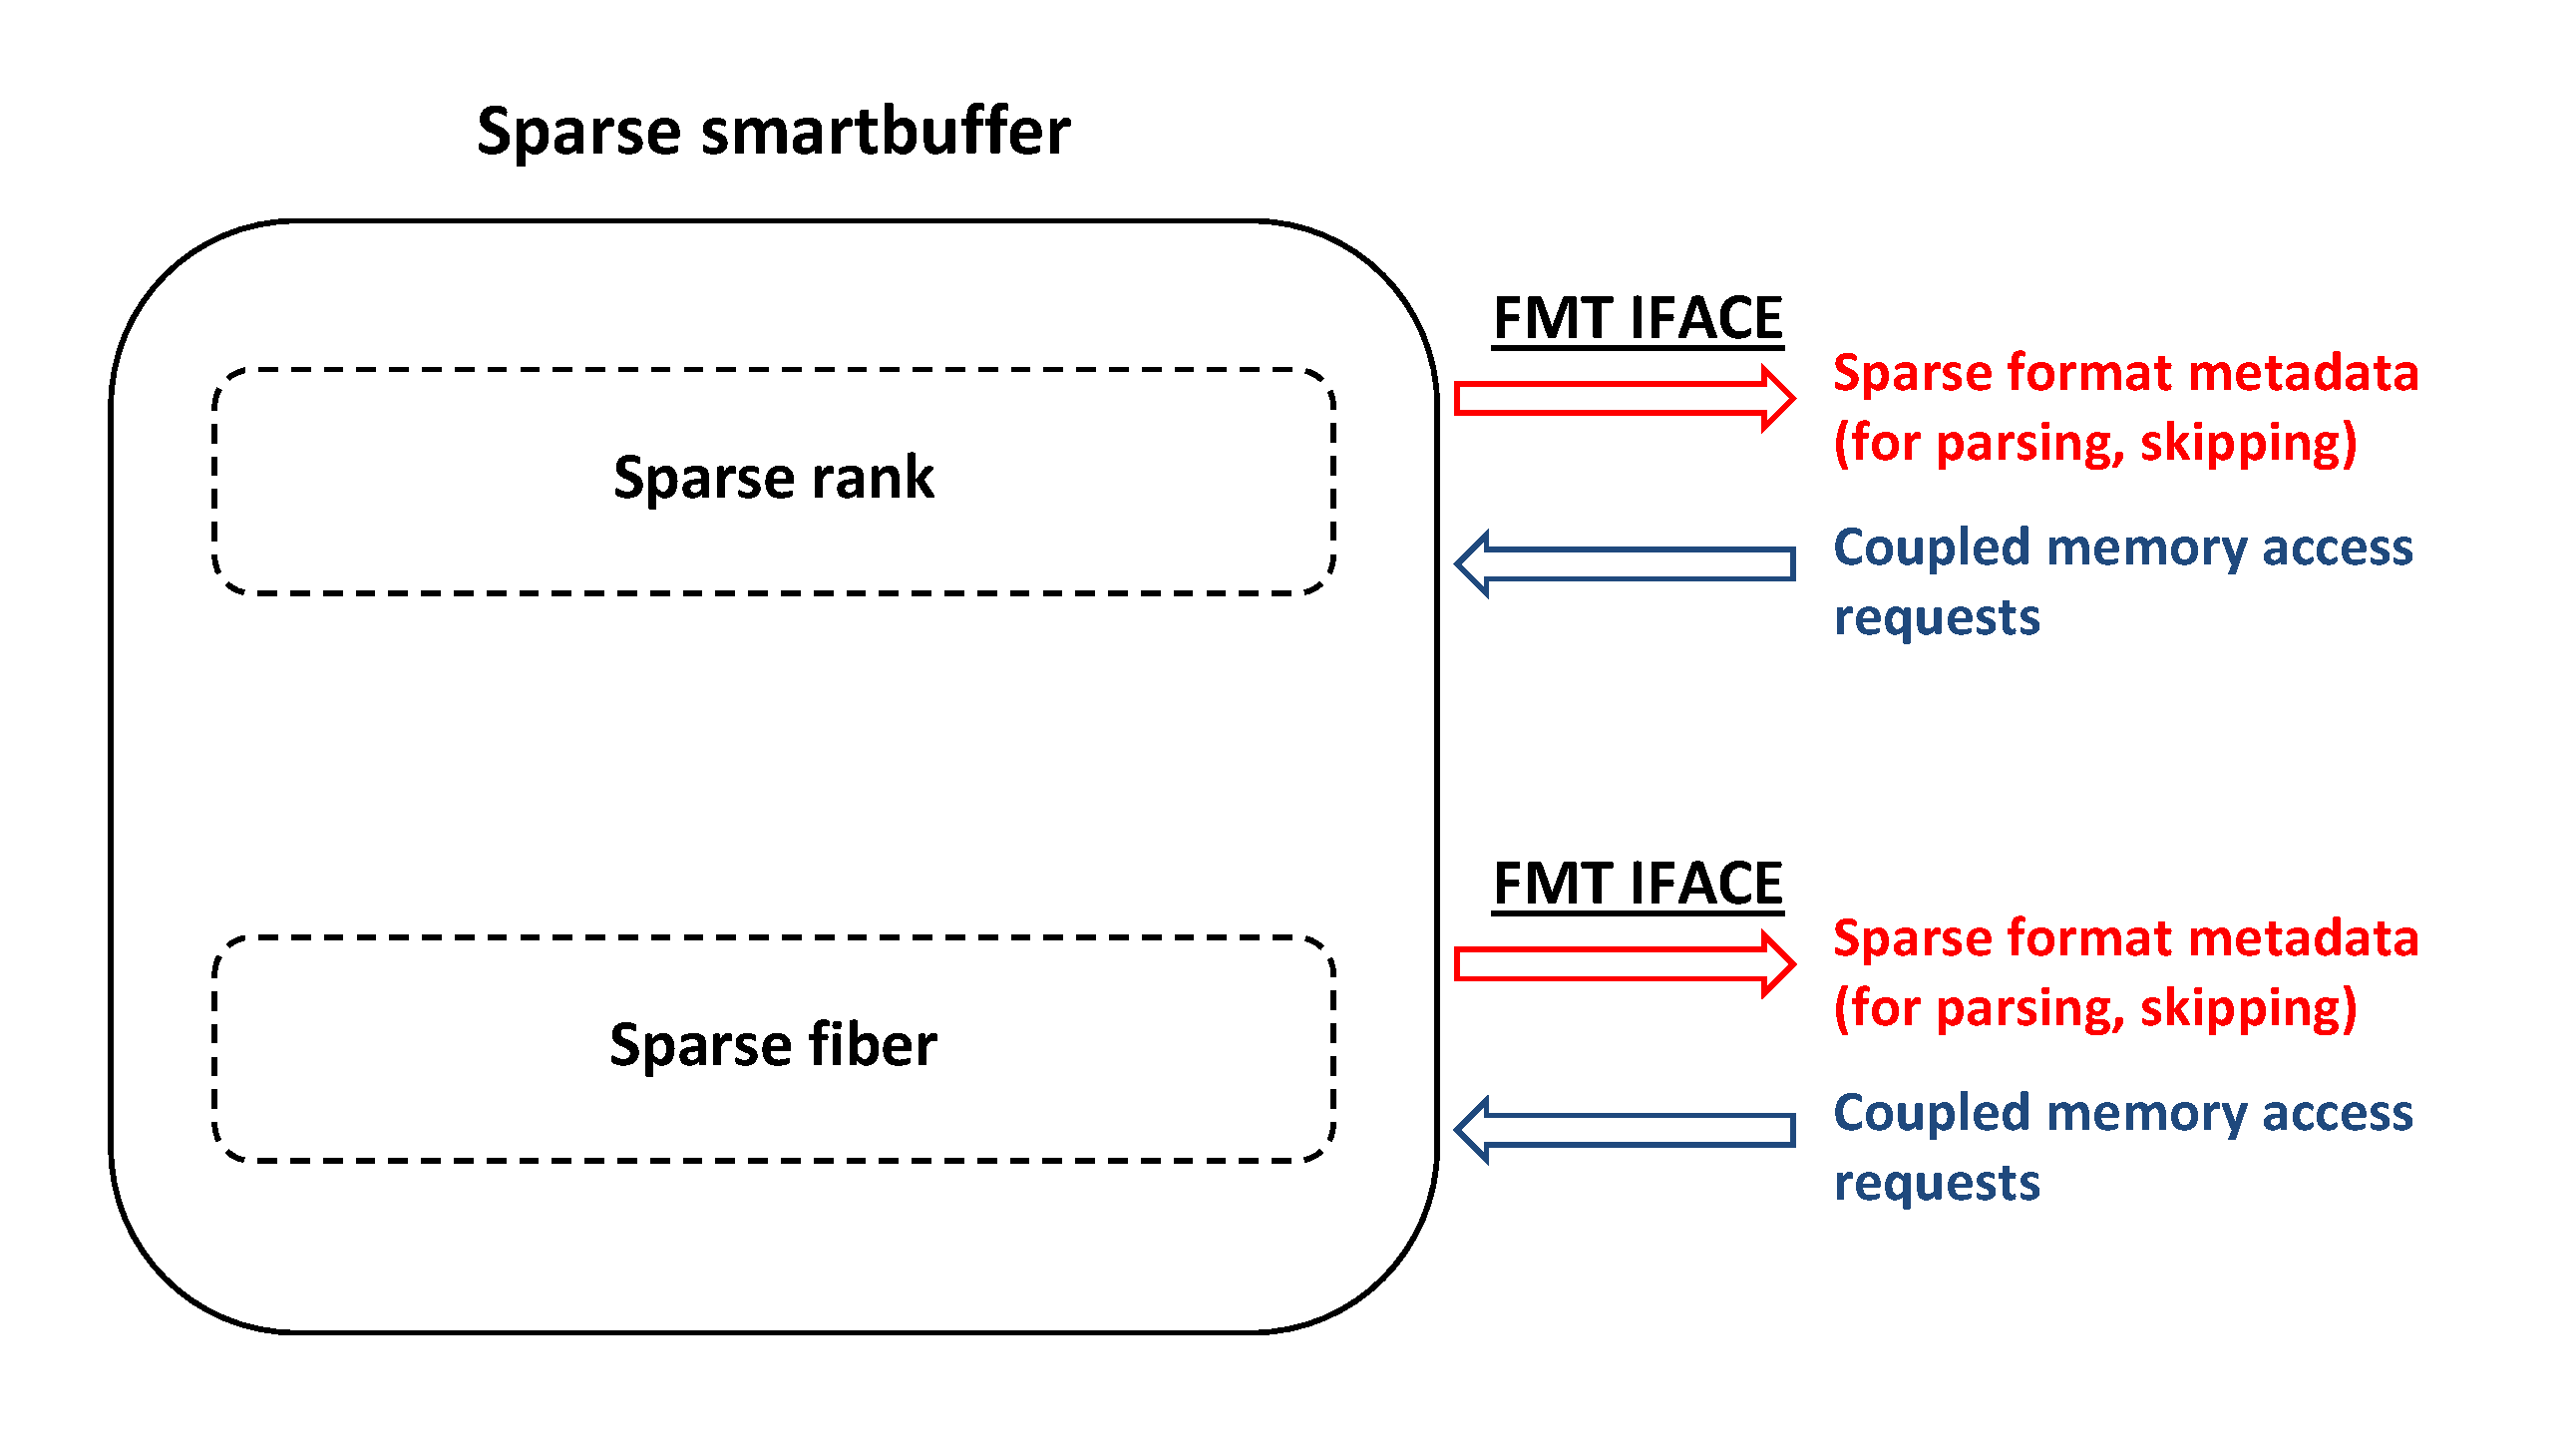
\includegraphics[width=0.95\textwidth]{figures/sparse_sbuff_overview.pdf}
    \caption{In this work, the details of memory implementation are encapsulated inside an abstract ``sparse smartbuffer'' with an identical IO bundle interface to each sparse rank. SAF microarchitecture can issue requests to a format interface in order to read a sparse rank's format metadata or trigger a payload read from a specified positional offset.}
    \label{fig:sparse_sbuff_overview}
\end{figure}

Each fibertree rank resident in the buffer, is hidden behind a format-agnostic IO bundle, called the ``format interface'' (fmt iface.) The format interface supports three operations:

\begin{itemize}
    \item \textbf{Get sparse fiber metadata:} Read a stream of sparse format metadata associated with one fiber in a given rank.
    \item \textbf{Request payload read at specified positional offset:} Coupled data orchestration is supported via input wires in the format interface IO bundle, which allow SAF microarchitecture to override the smartbuffer's internal decoupled data orchestration. Where EDDO data orchestration is desired, the format interface IO bundle inputs can simply be left unconnected.
    \item \textbf{Signal end-of-fiber:} Although \textit{Efficient Processing}\cite{szebook} focuses on EDDO data orchestration, some sparse dataflow microarchitectures proposed in the book have a limited amount of coupled data orchestration, in the form of one-bit flags which synchronously reset the otherwise decoupled sequence generators when the end of a fiber is reached. In this work, the format interface IO bundle includes a flag for signaling that the end of a fiber has been reached. The assumption here is that recognizing the end of a fiber may require specialized format metadata parsing within the SAF microarchitecture, and thus the format interface requires a flag input for the SAF microarchitecture to signal end-of-fiber to the rank's decoupled traversal logic.
\end{itemize}

Note the particular usage of ``encapsulation'' in this work: for the purposes of describing and modeling SAF microarchitecture, the internals of each sparse smartbuffer are not simply hidden behind the format interface, but rather are not implemented or modeled at all. The goal instead is to (1) define a consistent abstraction for the interface between architectural smartbuffers and SAF microarchitecture, and (2) define a set of \textit{workload boundary conditions} which are \textit{consistent} with sparse smartbuffer functionality under worst-case dataflow conditions. Here, \textit{workload} refers to any appropriate measure of the processing effort that is required of a SAF microarchitecture connected to the IO. Once the worst-case workload requirements are estimated for all format interfaces, then the SAF microarchitecture may be designed to satisfy the workload requirements, without regard to the overall dataflow. 

Figure~\ref{fig:sparse_sbuff_wkld_overview} provides a high-level overview of how workload boundary conditions are bound to format interfaces on a sparse smartbuffer. Note that all workload measures have a \textit{direction} which matches the IO they apply to. In Figure~\ref{fig:sparse_sbuff_wkld_overview}, the $w_{md}$ workloads (red) are bound to format interface output wires; $w_{md}$ is a measure of the processing effort imposed on the \textit{input port} of any SAF microarchitecture connected to the format interface output wires. The $w_{pos}$ workloads (blue) are bound to format interface input wires; $w_{pos}$ is a measure of the processing effort imposed on the \textit{output port} of any SAF microarchitecture connected to the format interface input wires.

\begin{figure}[ht]
    \centering
    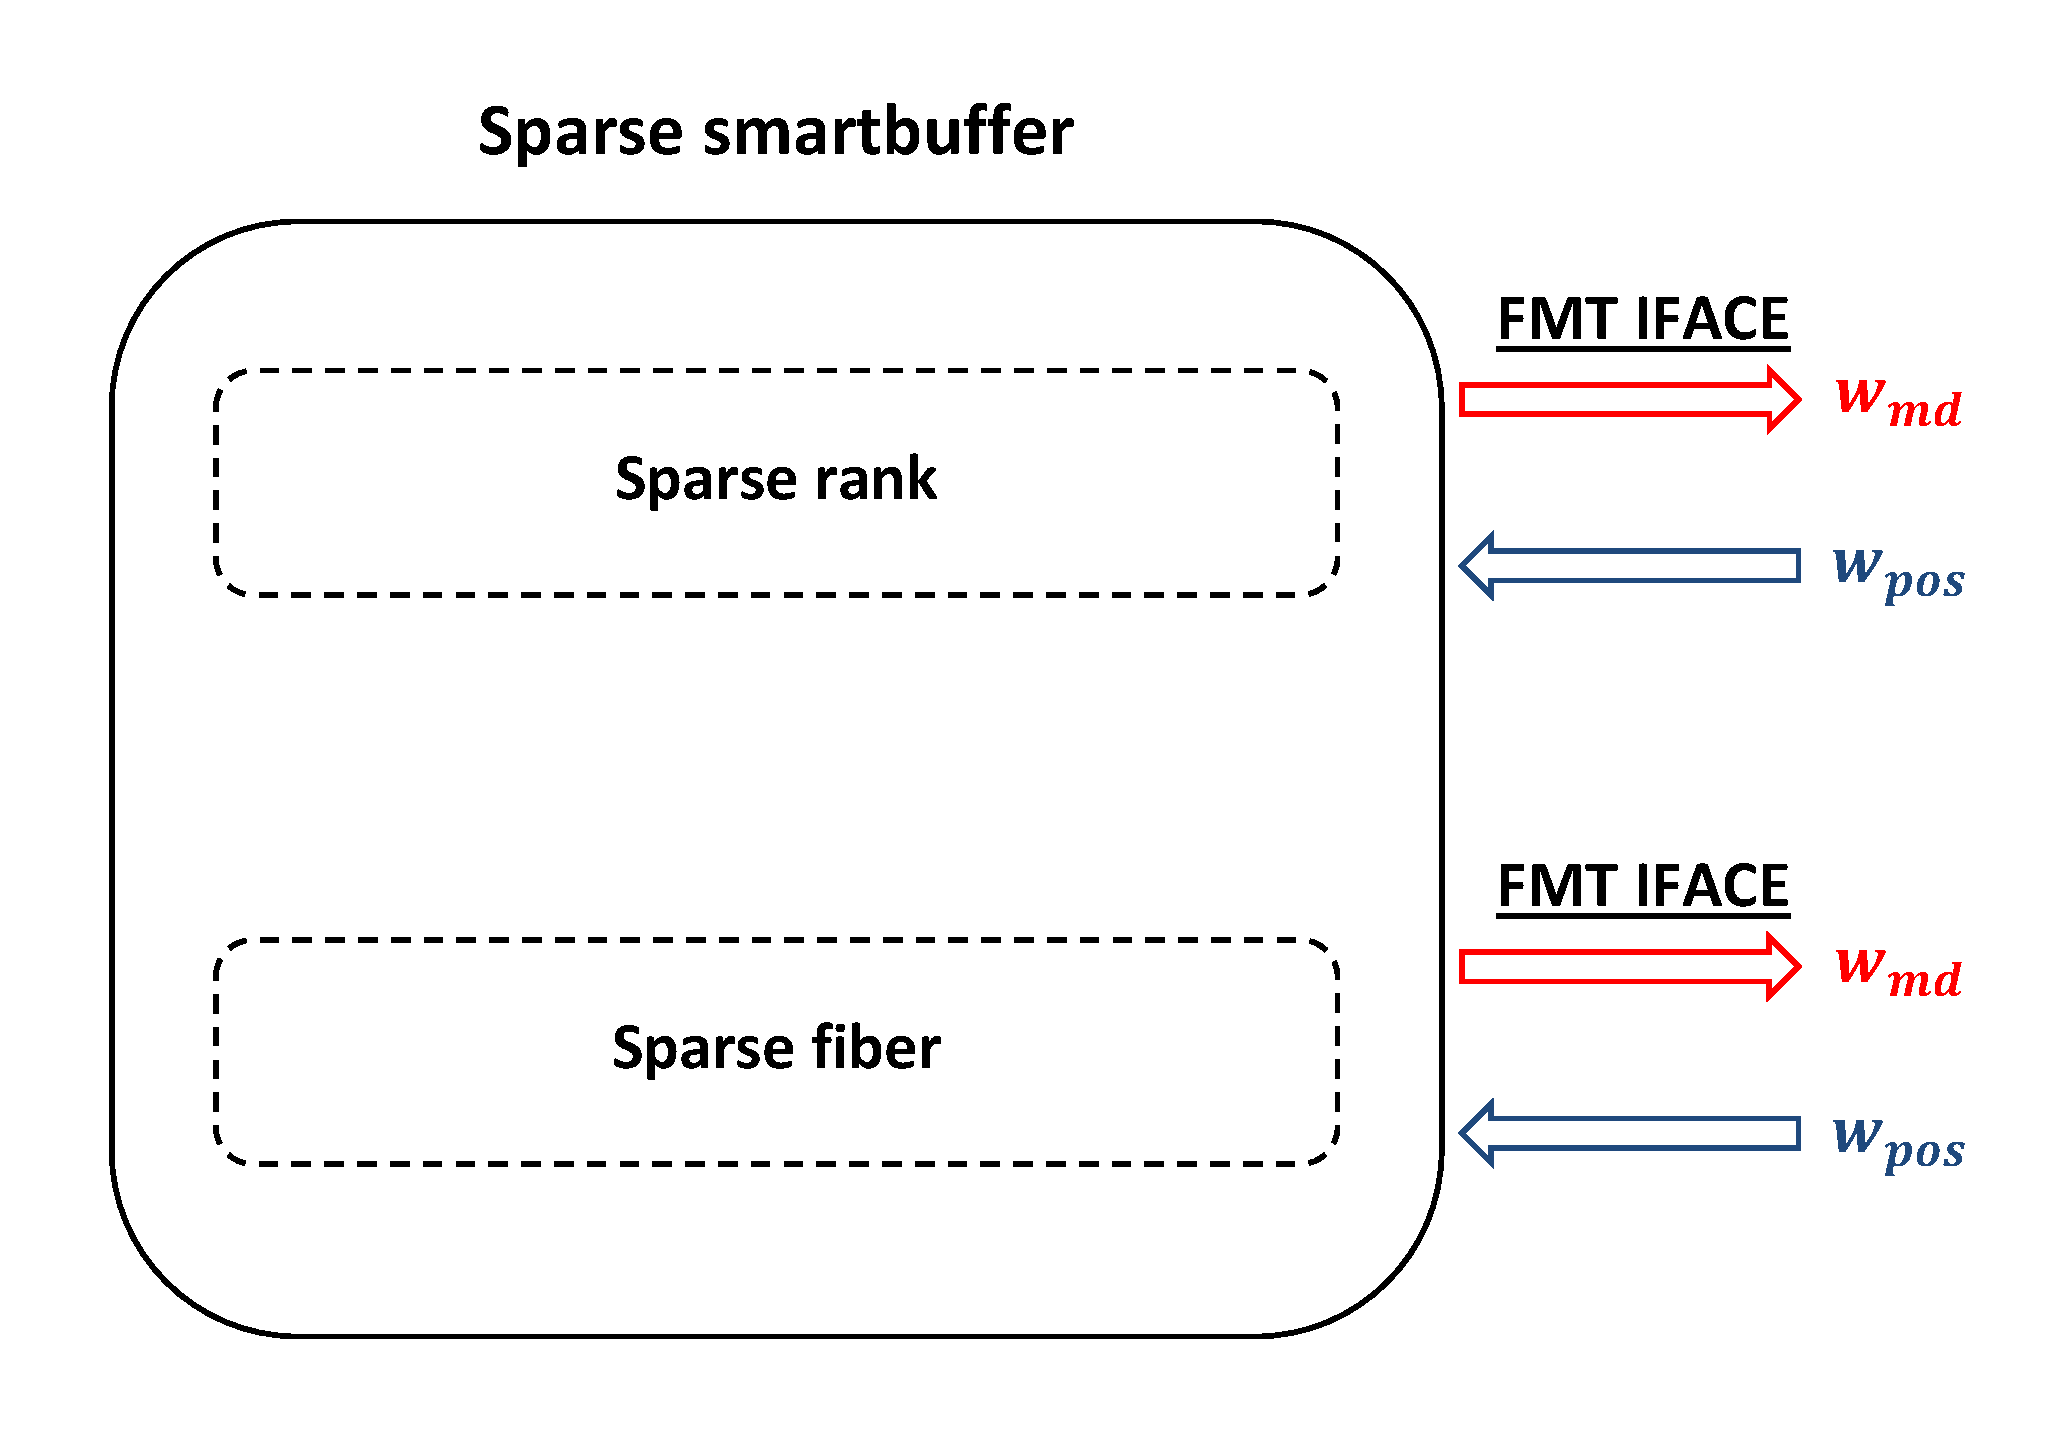
\includegraphics[width=0.95\textwidth]{figures/sparse_sbuf_wkld_overview.pdf}
    \caption{Sparse dataflow is abstracted behind \textit{workload boundary conditions}}.
    \label{fig:sparse_sbuff_wkld_overview}
\end{figure}

% Architecture, non-SAF microarchitecture, SAF microarchitecture



\subsection{Sparse smartbuffer model}

Although this work is not focused on modeling sparse smartbuffers, nonetheless it is helpful to develop a ``reference design'' for what a sparse smartbuffer implementation might look like. There are two reasons for this

\begin{itemize}
    \item \textbf{Define the format interface IO bundle.} Creating a sparse smartbuffer reference design helps us to be very concrete about what input and output wires a format interface must have, in order to support the most common workloads that operate on sparse fibers.
    \item \textbf{Workload modeling.} A mental model of sparse smartbuffer internals will be helpful later on when we bind workload measures to format interfaces.
\end{itemize}

This section will build up a reference design for a sparse smartbuffer in steps: (1) describe a single-fiber sparse smartbuffer for explicit-coordinate representation formats, (2) describe a single-fiber sparse smartbuffer for general explicit/implicit coordinate representation formats, and finally (3) describe a pipelined sparse smartbuffer capable of traversing a fibertree with support for general explicit/implicit coordinate representation formats.

\subsubsection{Composition}
\label{sec:composition}

A sparse smartbuffer can utilize some components which are familiar from dense smartbuffers\cite{buffet}\cite{sparseloop}, however, the sparse smartbuffer must have additional logic for operating on sparse fibers in order to correctly traverse a sparse fiber. Recall from Section~\ref{sec:what_is_a_saf_microarchitecture} that a SAF microarchitecture refers to that subset of an accelerator's microarchitecture, which either (1) was designed for processing sparse representation formats, or (2) is critical for the accelerator to correctly process sparse representation formats. This work is focused on describing and modeling SAF microarchitectures; since we ultimately are not striving to model smartbuffer internals, it is desirable to completely decouple the smartbuffer's sparse format processing logic into a separate component.

\begin{figure}[ht]
    \centering
    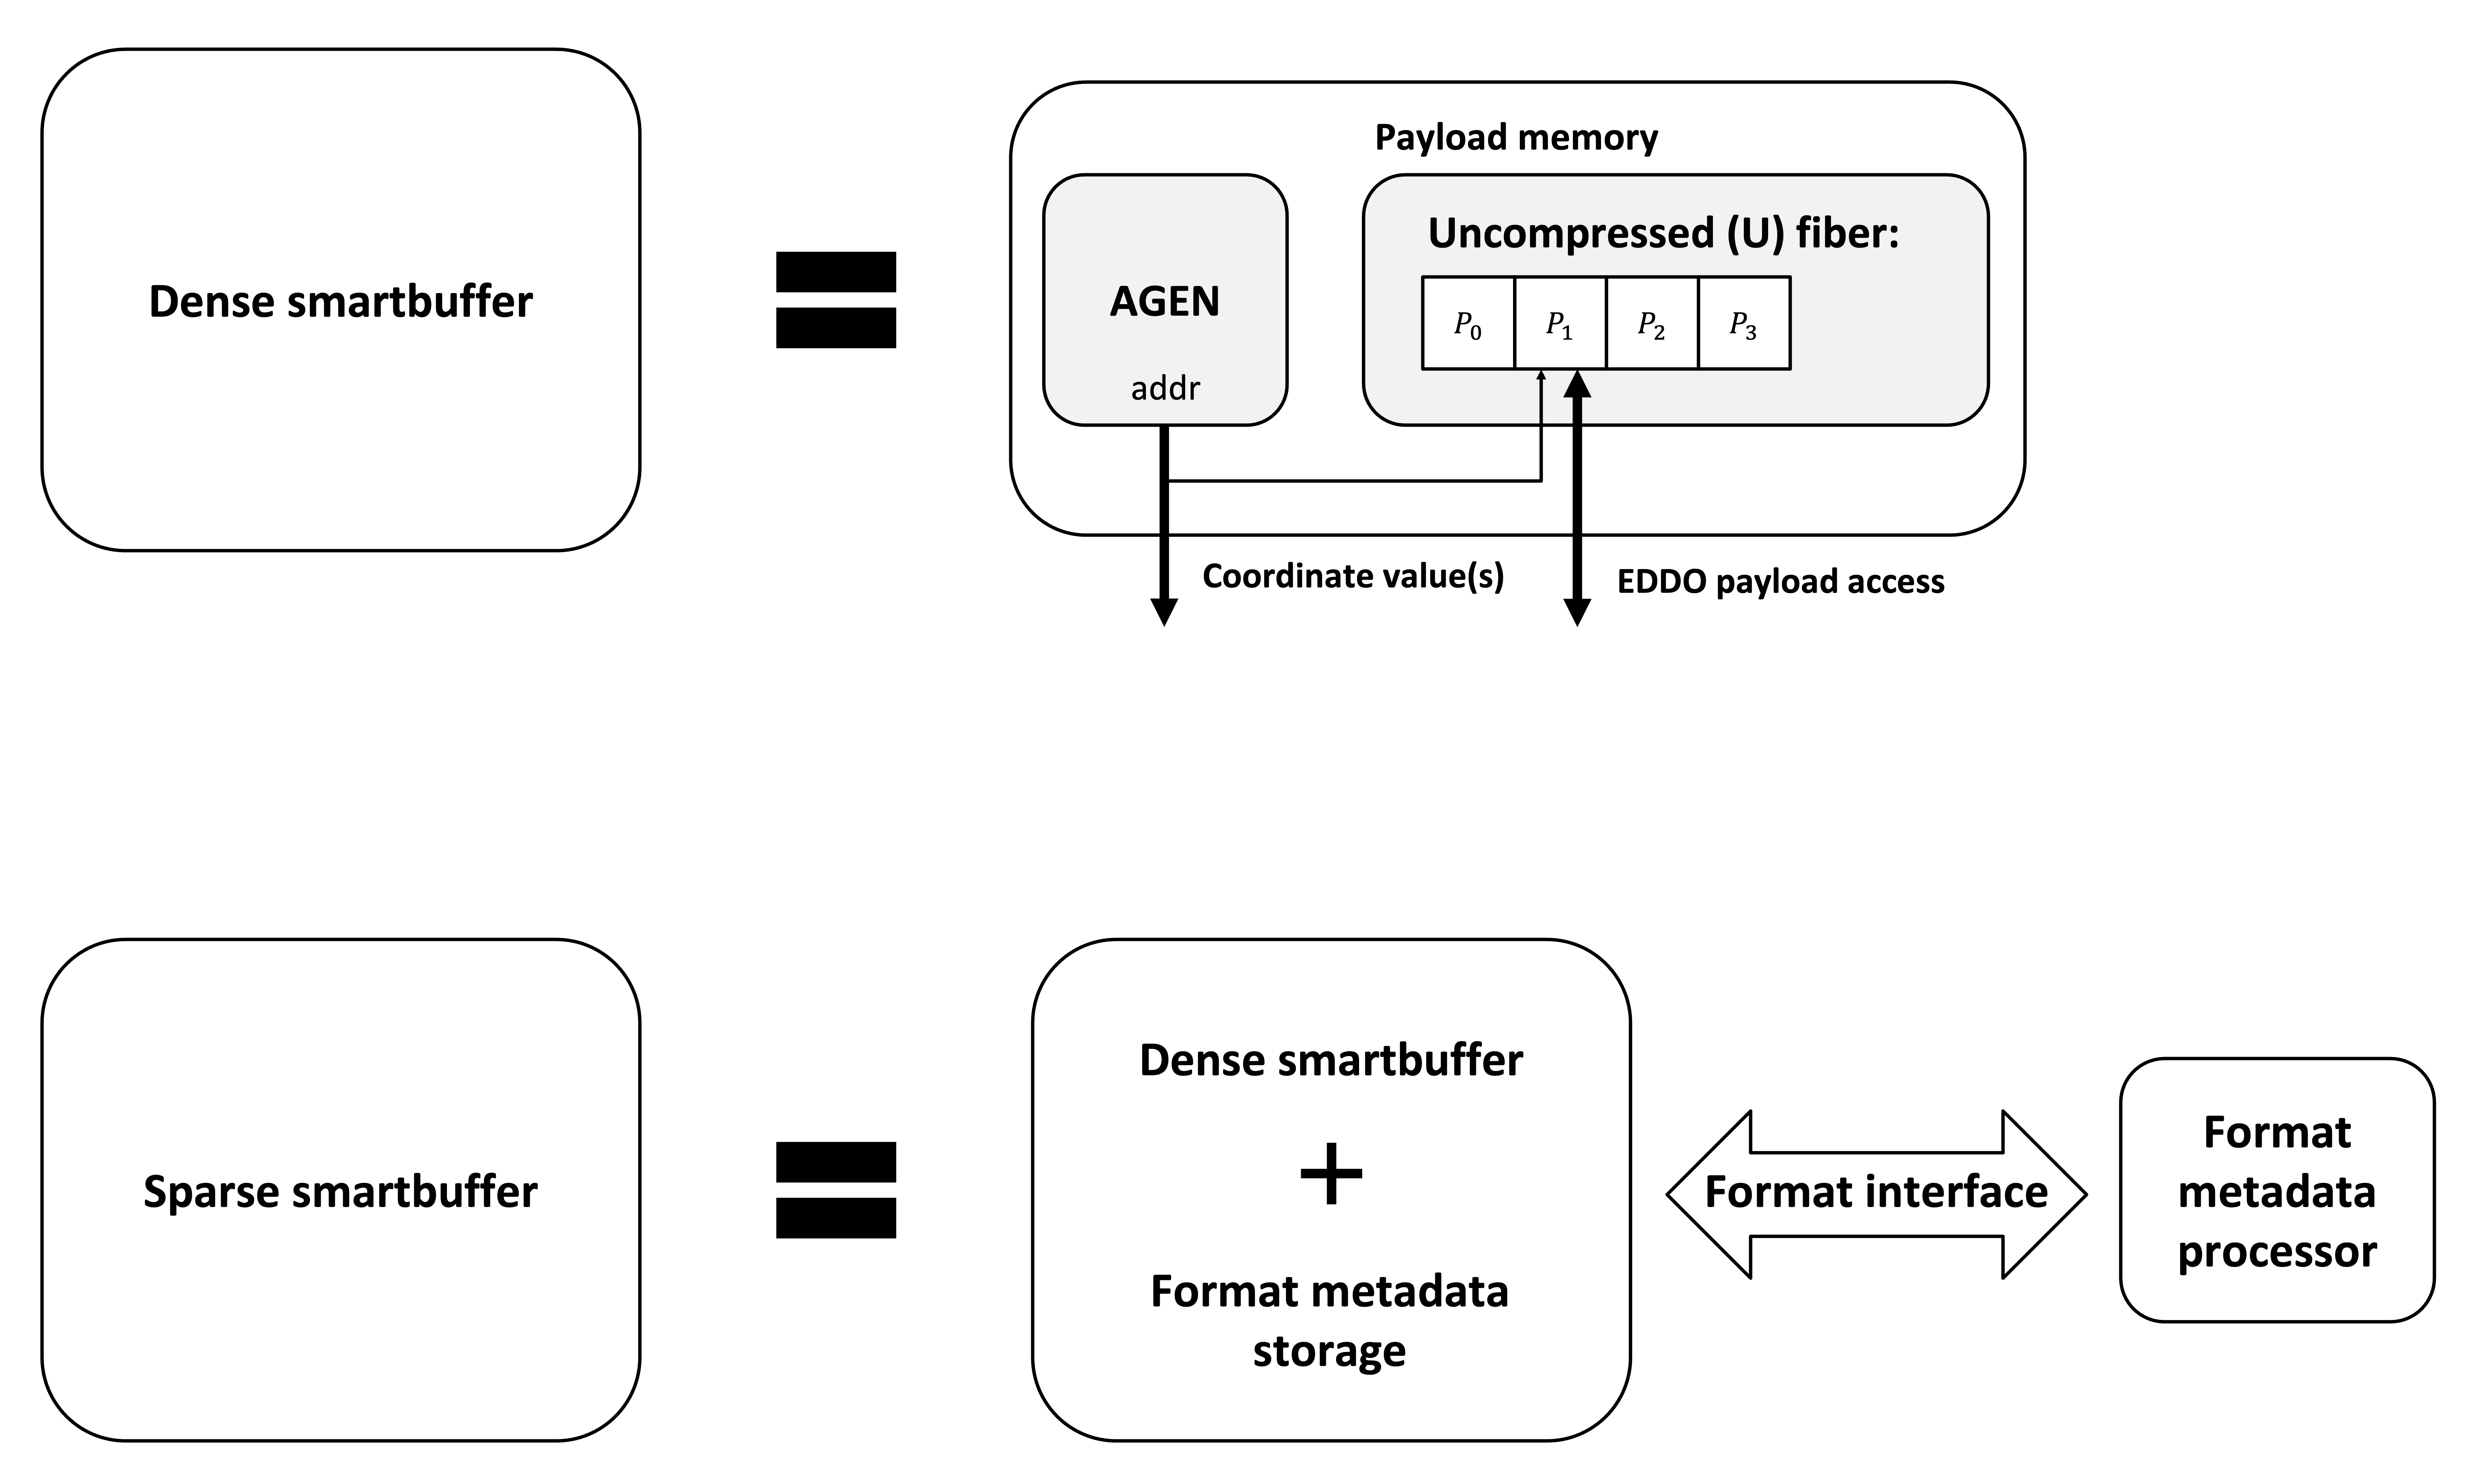
\includegraphics[width=0.95\textwidth]{figures/dense_smartbuffer_composition.png}
    \caption{This work models a \textit{sparse smartbuffer} as the composition of a dense smartbuffer with additional hardware that handles the compressed sparse tensor format, connected by an I/O bundle (``format interface''.) The format interface moves sparse format metadata from the dense smartbuffer metadata storage to the format metadata processor, and moves control signals in the other direction.}
    \label{fig:dense_smartbuffer_composition}
\end{figure}

Figure~\ref{fig:dense_smartbuffer_composition} (\textit{bottom}) shows how the sparse smartbuffer is modeled as a dense smartbuffer (\textit{top}) composed with (1) additional storage for sparse format metadata, and (2) a SAF microarchitecture that can process sparse format metadata. 

The dense smartbuffer in Figure~\ref{fig:dense_smartbuffer_composition} (\textit{top}) only holds one fiber; the AGEN unit implements decoupled fiber traversal by generating a stream of coordinate values which lookup into the uncompressed fiber (position and coordinate are synonymous for an uncompressed fiber.)

When the smartbuffer is storing a compressed sparse fiber, it becomes reliant on the SAF microarchitecture to receive sparse format metadata that is output through the format interface, and to send back control signals which ensure correct traversal.

\subsubsection{Single-rank, explicit-coordinate-format sparse smartbuffer model}
\label{sec:single_explicit_fiber}

Building on Section~\ref{sec:composition}, we can flesh out how the sparse smartbuffer internals and the format interface might be designed if the sparse fiber uses an explicit coordinate\cite{szebook} format such as coordinate-payload (C)\cite{szebook}.

\begin{figure}[ht]
    \centering
    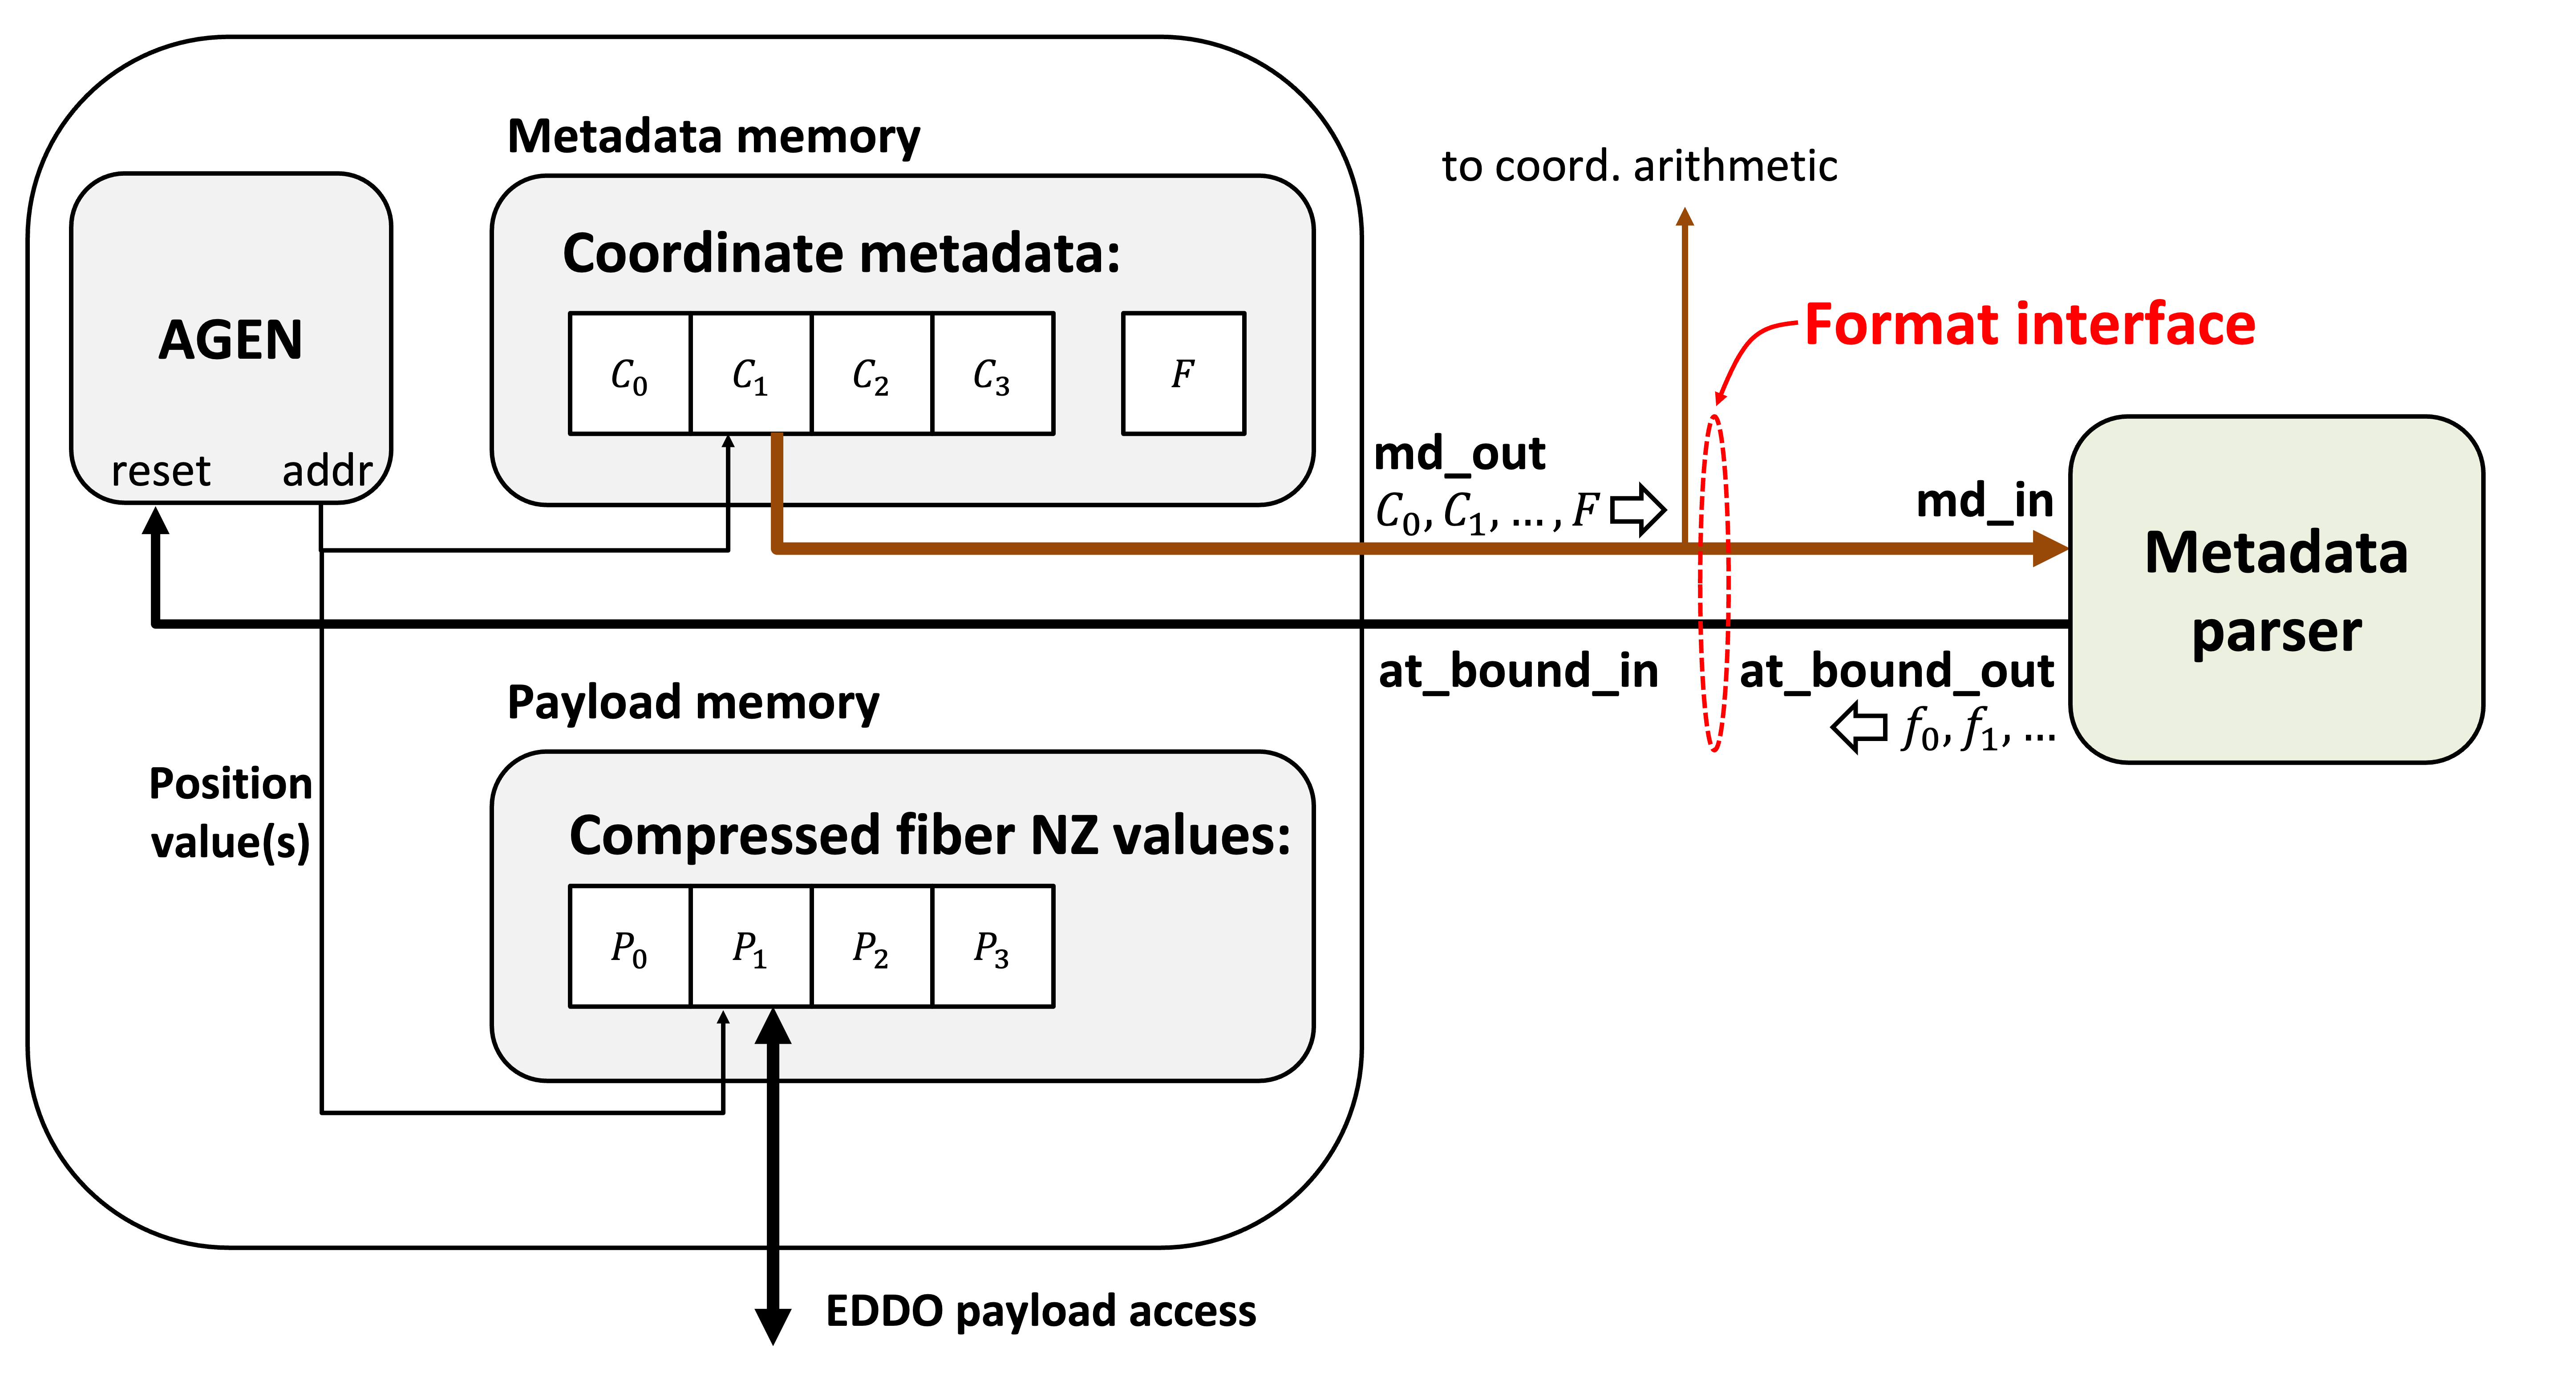
\includegraphics[width=0.95\textwidth]{figures/single_rank_explicit_coordinate_smartbuffer_model.png}
    \caption{Sparse smartbuffer model for a single rank, supporting explicit coordinate sparse tensor formats. ${C_i}$ are explicit coordinate metadata values. $F$ is a stand-in for any metadata regarding fiber characteristics, i.e. number-of-non-zeros. ${f_i}$ are flag values - metadata parser parses metadata arriving at md\_in and sets at\_bound\_out when fiber traversal is complete.}
    \label{fig:single_rank_explicit_coordinate_smartbuffer_model}
\end{figure}

In the coordinate-payload format, each non-zero/non-empty payload is paired with a coordinate metadata value. Figure~\ref{fig:single_rank_explicit_coordinate_smartbuffer_model} shows how the address generator implements traversal by looking up corresponding elements in the \textit{coordinate metadata} and \textit{compressed fiber non-zero (NZ) values} arrays. 

The only role for the metadata parser is to detect when the entirety of the fiber has been processed, and send a reset signal back over the format interface in order reset the traversal. Thus, the format interface consists simply of

\begin{itemize}
    \item \textbf{md\_out (output):} Output a stream of explicit coordinates to the metadata parser.
    \item \textbf{at\_bound\_in (input):} Receive the reset signal from the metadata parser upon completing fiber traversal.
\end{itemize}

\subsubsection{Single-rank, general-format sparse smartbuffer model}

It becomes apparent that the format interface and reference design in Section~\ref{sec:single_explicit_fiber}, while sufficient for an explicit-coordinate sparse format, are insufficient for an implicit-coordinate sparse format such as bitmask (B)\cite{szebook}.

\begin{figure}[ht]
    \centering
    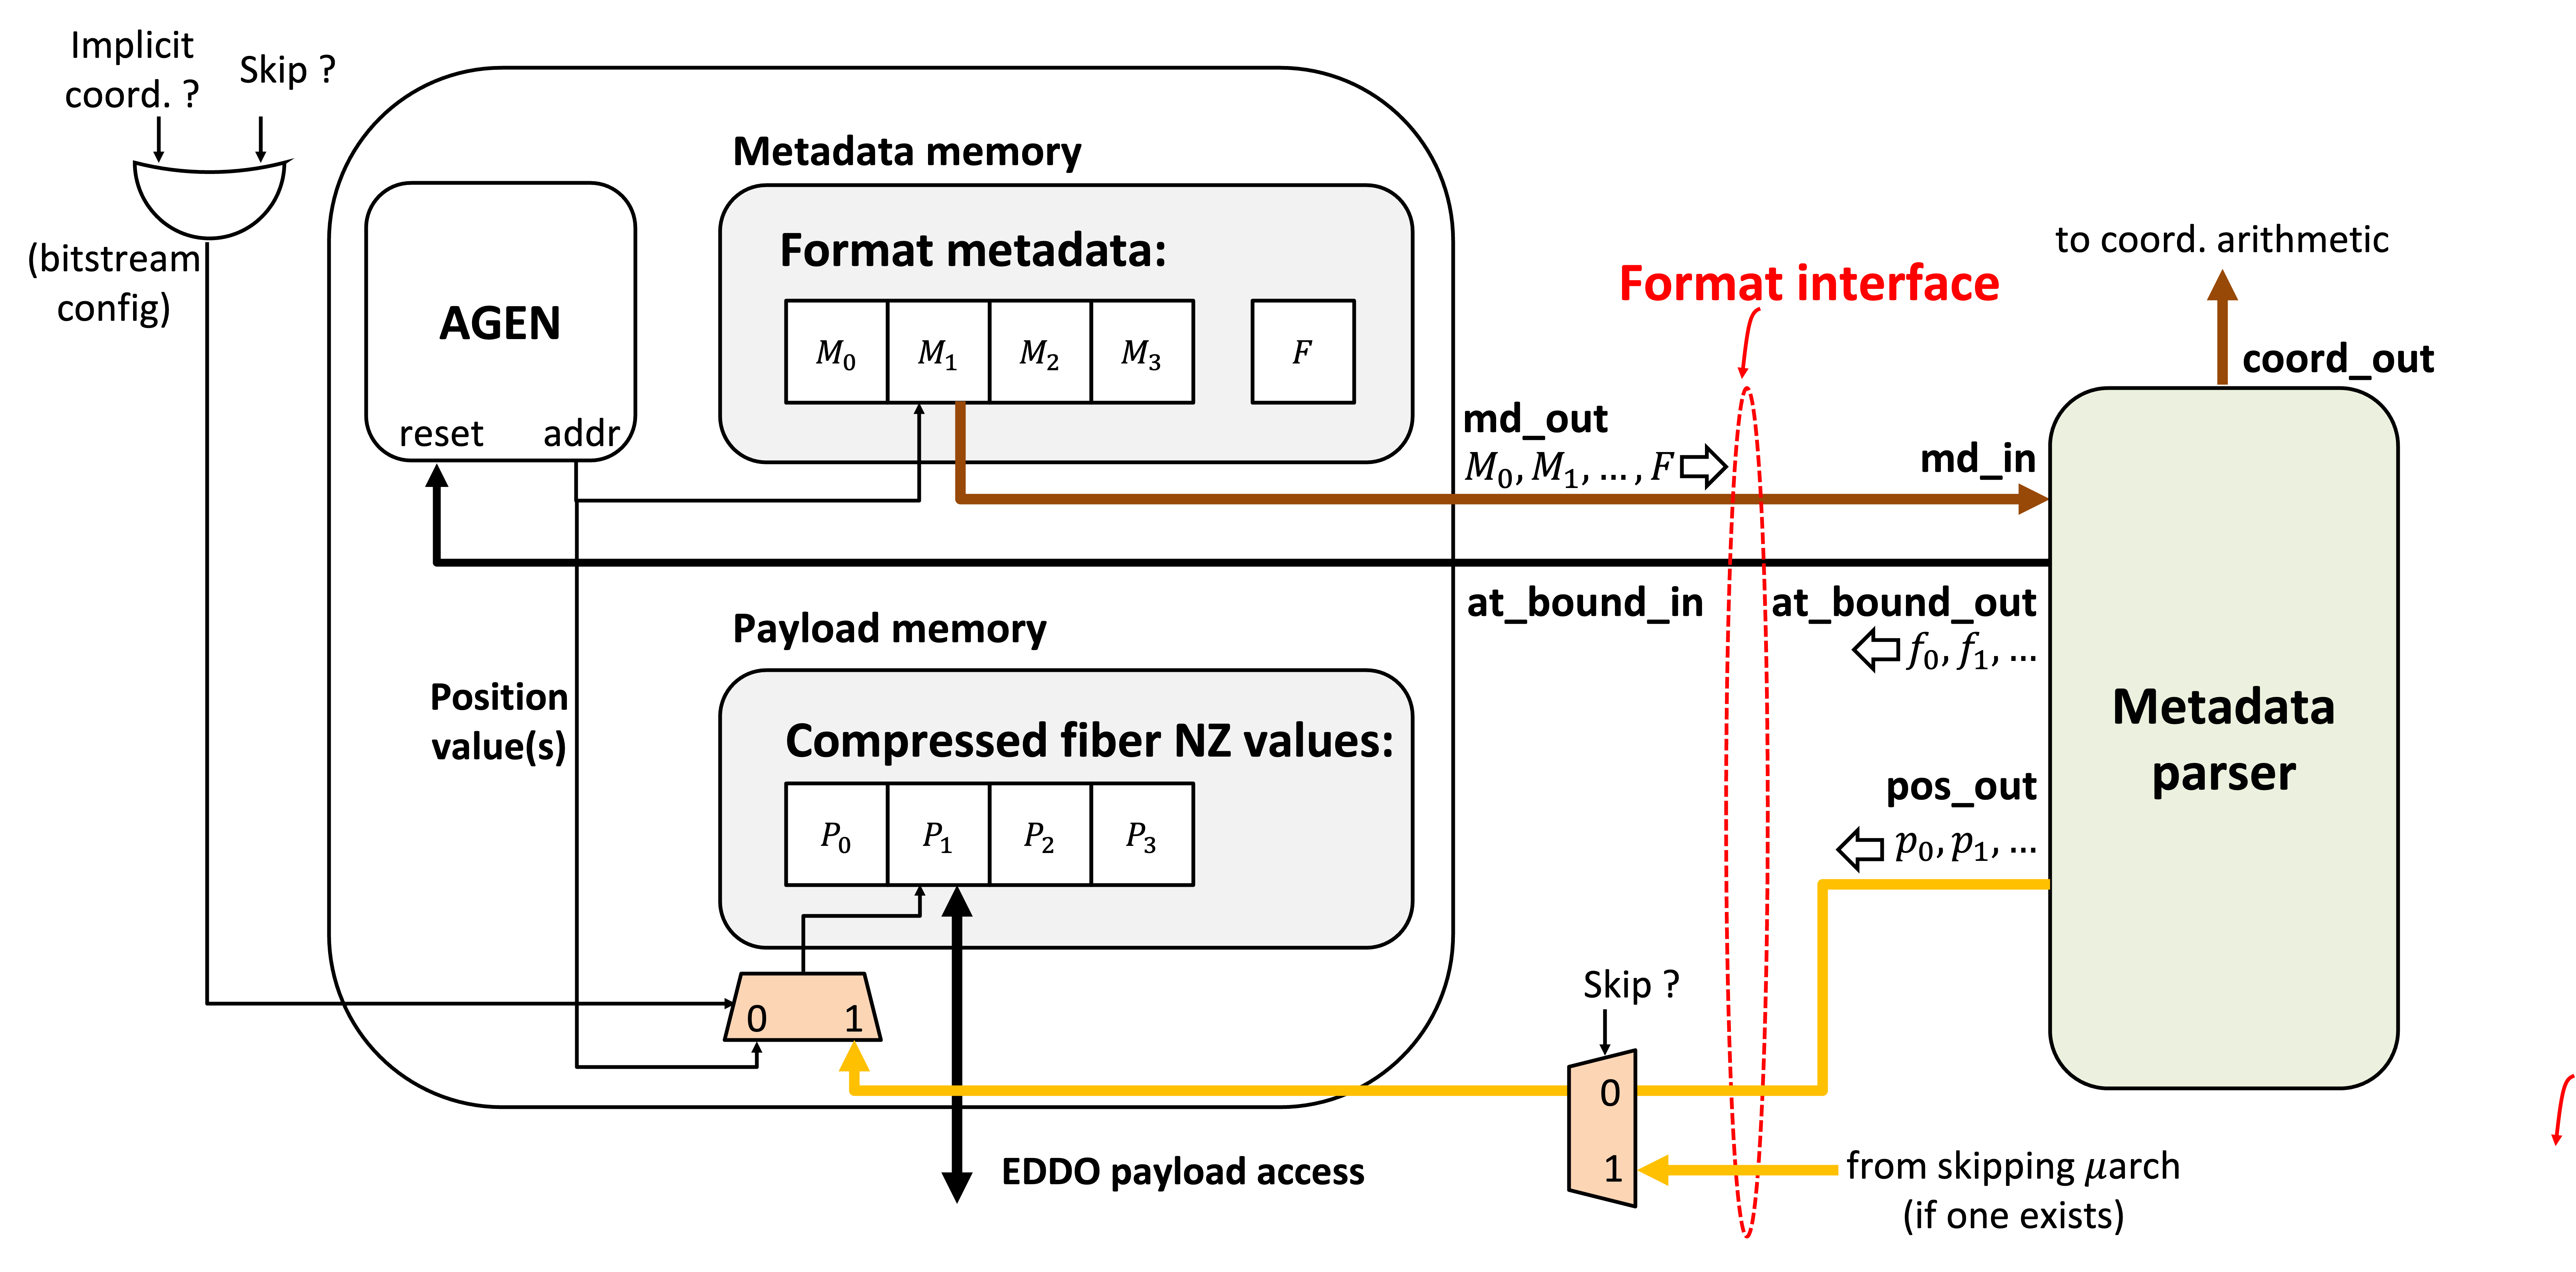
\includegraphics[width=0.95\textwidth]{figures/single_rank_general_format_smartbuffer_model.png}
    \caption{Sparse smartbuffer model for a single rank, supporting general sparse tensor formats. ${M_i}$ are general sparse metadata values, which may not be explicit coordinates. The metadata parser can orchestrate payload reads (via pos\_out) if this is enabled in the configuration bitstream. This is necessary for implicit coordinate representation formats. If skipping is enabled in the configuration bitstream, a skipping microarchitecture's output position stream can orchestrate payload reads. The functionality of the at\_bound\_out signal is unchanged. }
    \label{fig:single_rank_general_format_smartbuffer_model}
\end{figure}

There are a few problems with trying to apply the design in Figure~\ref{fig:single_rank_explicit_coordinate_smartbuffer_model} to a B-formatted fiber:

\begin{itemize}
    \item While B still stores the compressed fiber payloads as a series of consecutive non-zero/non-empty elements, the B-format metadata array always has a length equal to the dense length of the fiber's underlying rank, regardless of the number of non-zeroes. This prevents the AGEN from trivially co-iterating through the format-metadata and compressed-NZ-values arrays, as was done in Section~\ref{sec:single_explicit_fiber}.
    \item The B-format metadata may not be \textit{directly} utilized to lookup into the compressed-NZ-values array, as the metadata does not explicitly contain positional offsets that can be used for the lookup. 
\end{itemize}

In order to even look up into the compressed-fiber-NZ values, Figure~\ref{fig:single_rank_general_format_smartbuffer_model} shows that a different design is required which allows the metadata parser to process the B-format metadata into positional offsets and then request lookups into the compressed-fiber-NZ-values array. It is clear from Figure~\ref{fig:single_rank_general_format_smartbuffer_model} that the format interface bundle described in Section~\ref{sec:single_explicit_fiber} must be augmented with an additional input wire, which can receive requests from the metadata parser to lookup payloads in the compressed-fiber-NZ-values array.

\paragraph{Skipping.} 

\subsubsection{Multi-rank-pipelined (hierarchical), general-format sparse smartbuffer model}

\begin{figure}[ht]
    \centering
    \includegraphics[width=0.95\textwidth]{figures/hierarchical_general_format_sparse_smartbuffer.png}
    \caption{A sparse smartbuffer that stores a multi-rank tensor, inspired by the ExTensor\cite{extensor} design for traversing and intersecting deep fibertrees. The format microarchitecture implements a rank-parallel metadata processing pipeline. See Figure~\ref{fig:format_interface} for the structure of the format interface I/O bundle.}
    \label{fig:hierarchical_general_format_sparse_smartbuffer}
\end{figure}

\begin{figure}[ht]
    \centering
    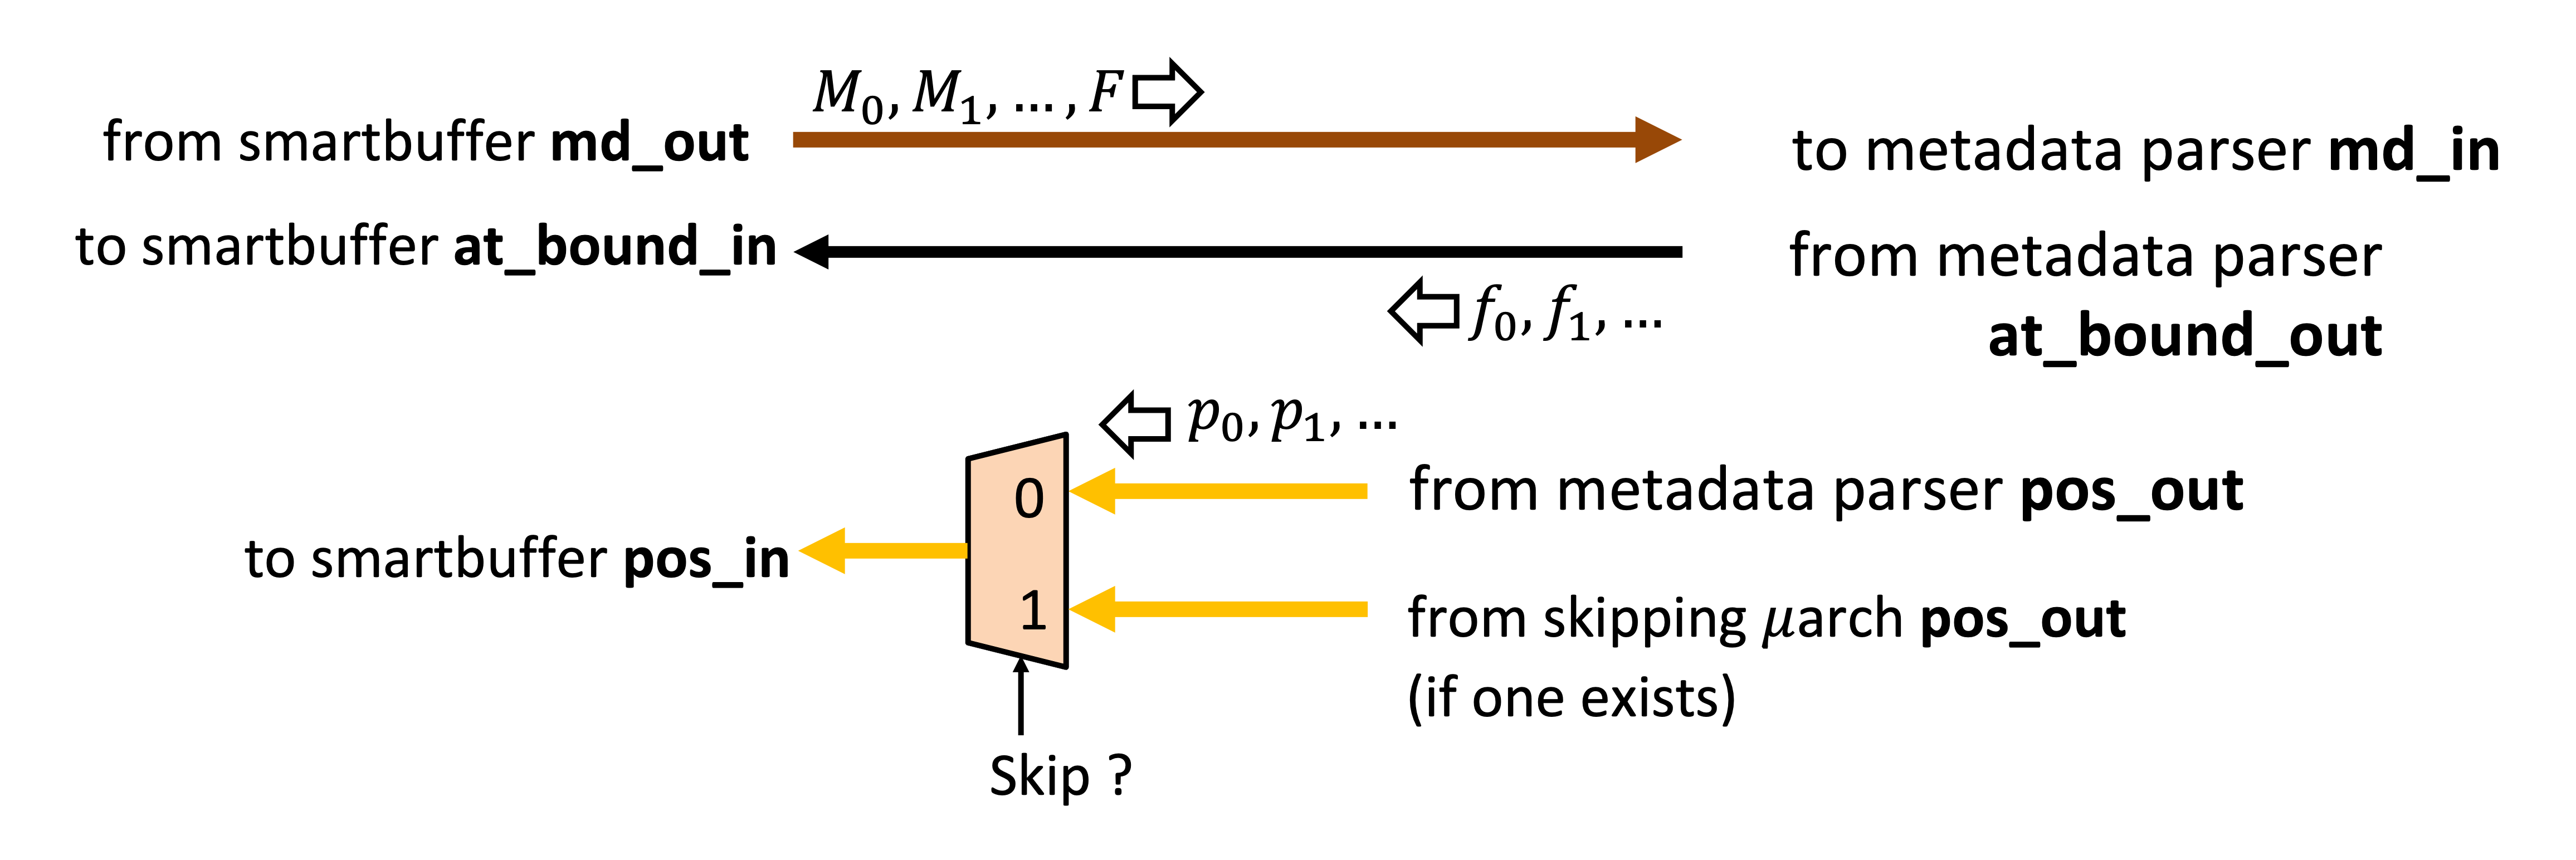
\includegraphics[width=0.95\textwidth]{figures/format_interface.png}
    \caption{Format interface I/O bundle. Sparse metadata moves from md\_out to md\_in. Payload lookup address offsets move from pos\_out to pos\_in. at\_bound\_out signals that fiber traversal is complete. The MUX that switches pos\_in between the metadata parser and the skipping microarchitecture is technically not part of the I/O bundle but is included for clarity and context.}
    \label{fig:format_interface}
\end{figure}

\subsection{Component parameterization}



\section{Integrating prior work}

\subsection{Unified skipping microarchitecture abstraction}

\begin{figure}[ht]
    \centering
    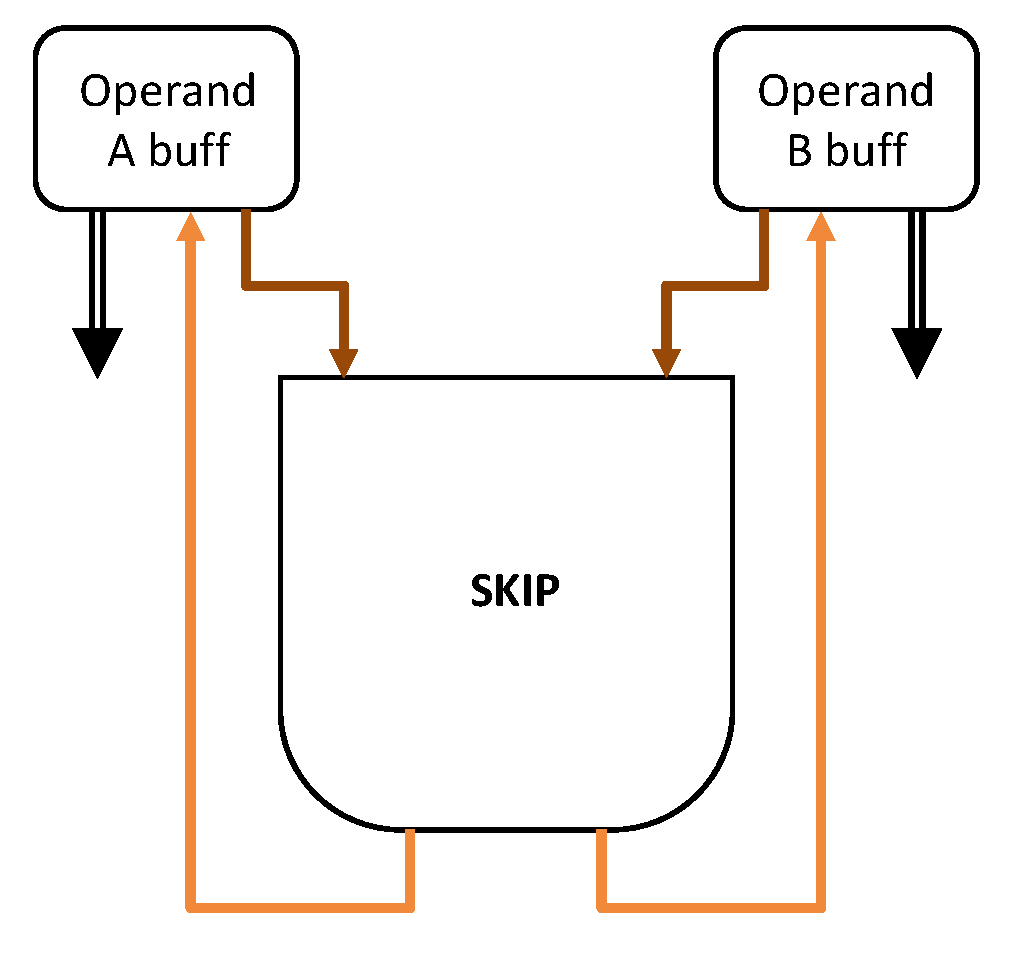
\includegraphics[width=0.7\textwidth]{figures/uniform_skip_topo.pdf}
    \caption{The unified skipping microarchitecture abstraction.}
    \label{fig:uniform_skip_topo}
\end{figure}

\subsubsection{Elaborating leader-follower skipping microarchitecture}

\begin{figure}[ht]
    \centering
    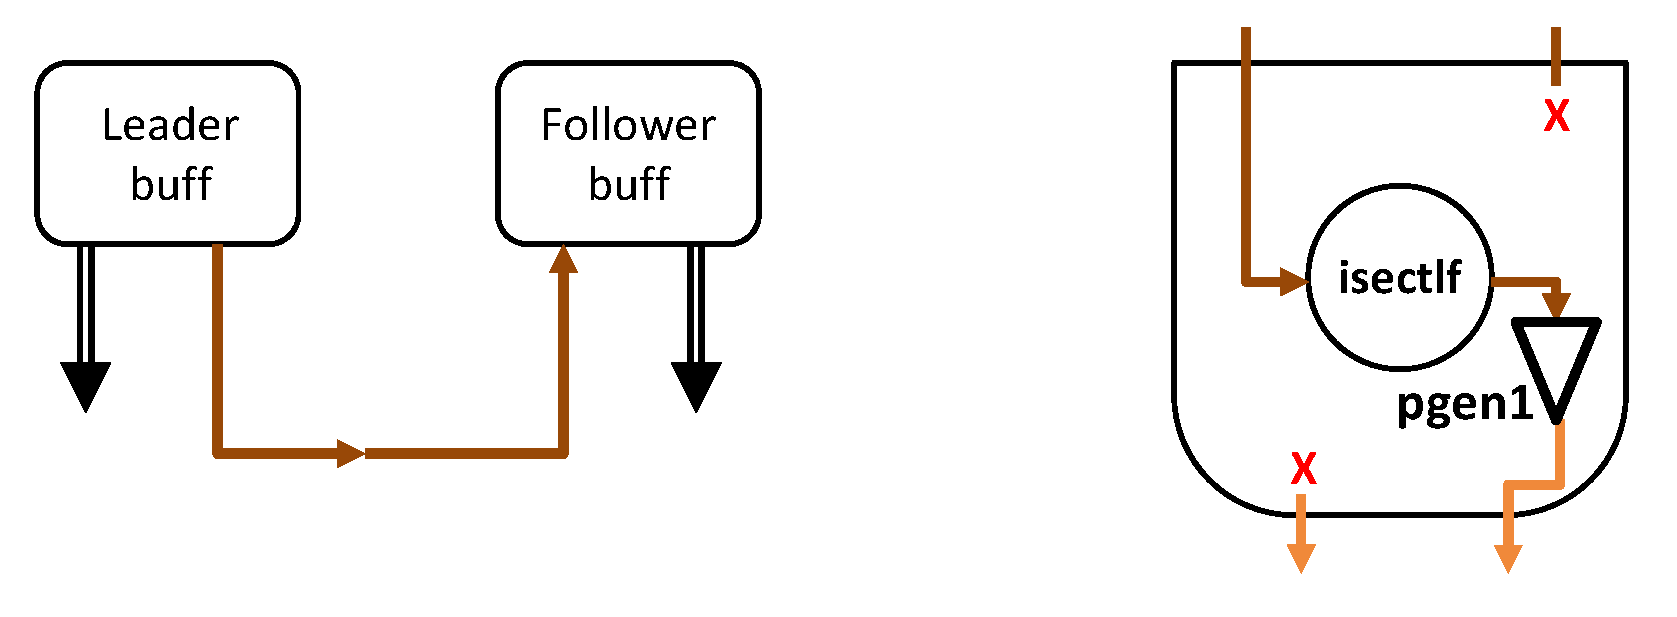
\includegraphics[width=0.7\textwidth]{figures/prior_lf_skip.pdf}
    \caption{Inferring leader-follower skipping microarchitecture topology.}
    \label{fig:prior_lf_skip}
\end{figure}

\subsubsection{Elaborating bidirectional skipping microarchitecture}

\begin{figure}[ht]
    \centering
    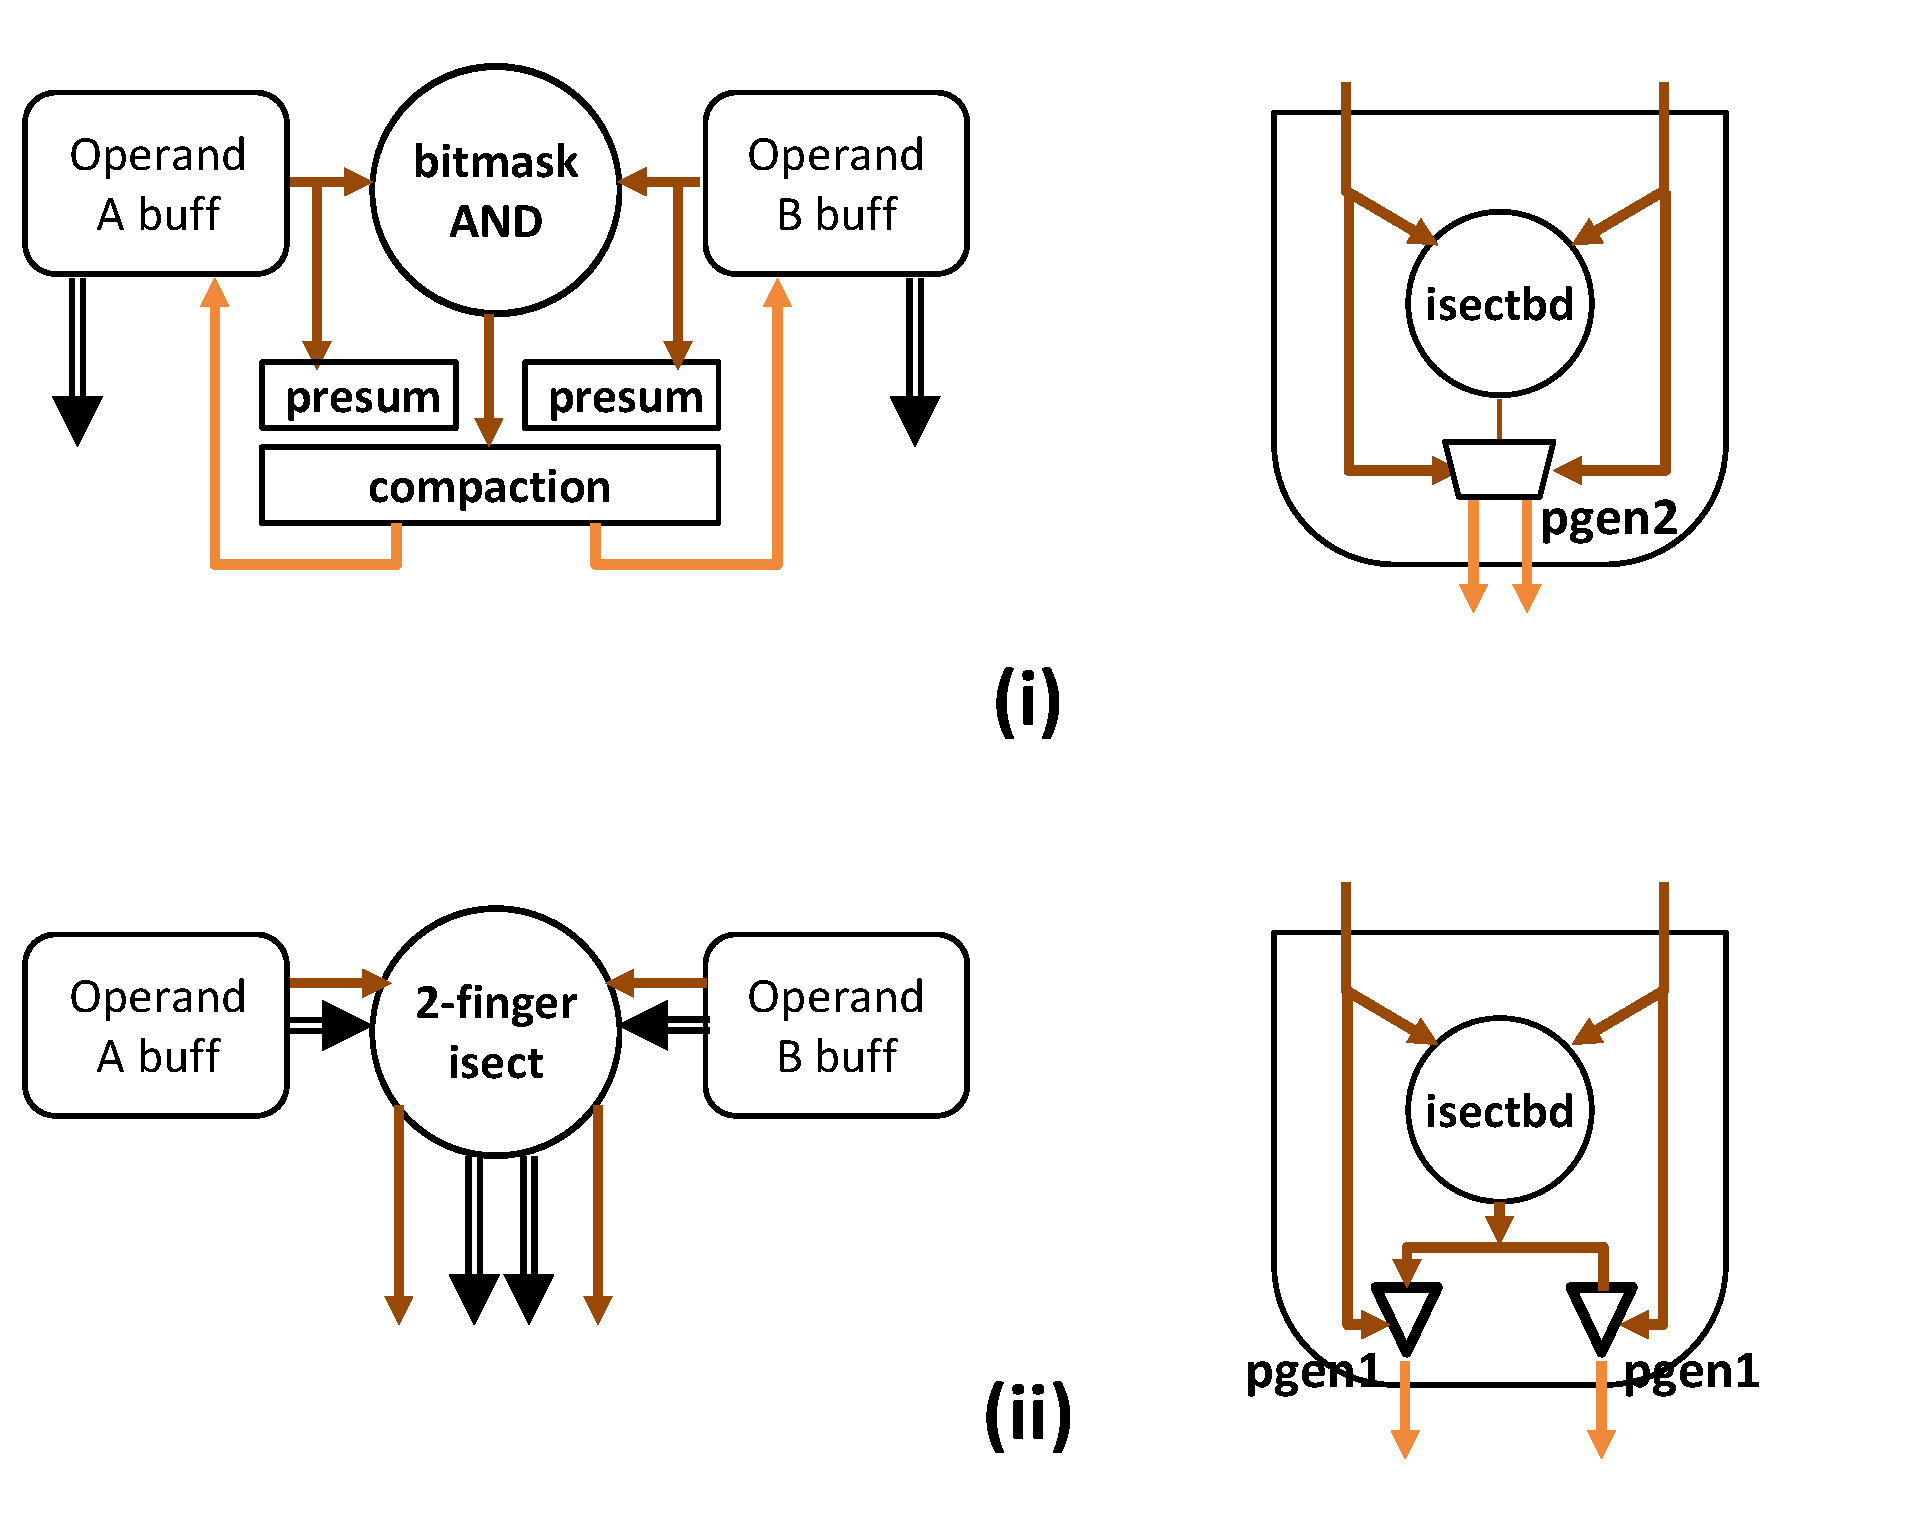
\includegraphics[width=0.95\textwidth]{figures/prior_bd_skip.pdf}
    \caption{Inferring bidirectional skipping microarchitecture topology.}
    \label{fig:prior_bd_skip}
\end{figure}

\subsection{Fill optimization}

\begin{figure}[ht]
    \centering
    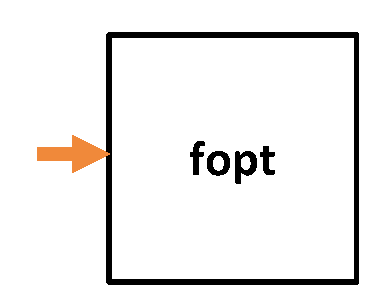
\includegraphics[width=0.6\textwidth]{figures/uniform_fopt.pdf}
    \caption{Unified Fill Optimizer SAF microarchitecture primitive.}
    \label{fig:uniform_fopt}
\end{figure}

\begin{figure}[ht]
    \centering
    
\includegraphics[width=0.6\textwidth]{figures/leader_lut.pdf}
    \caption{GAMMA\cite{gamma}-style LUT-based fill optimization.}
    \label{fig:leader_lut}
\end{figure}

\begin{figure}[ht]
    \centering
    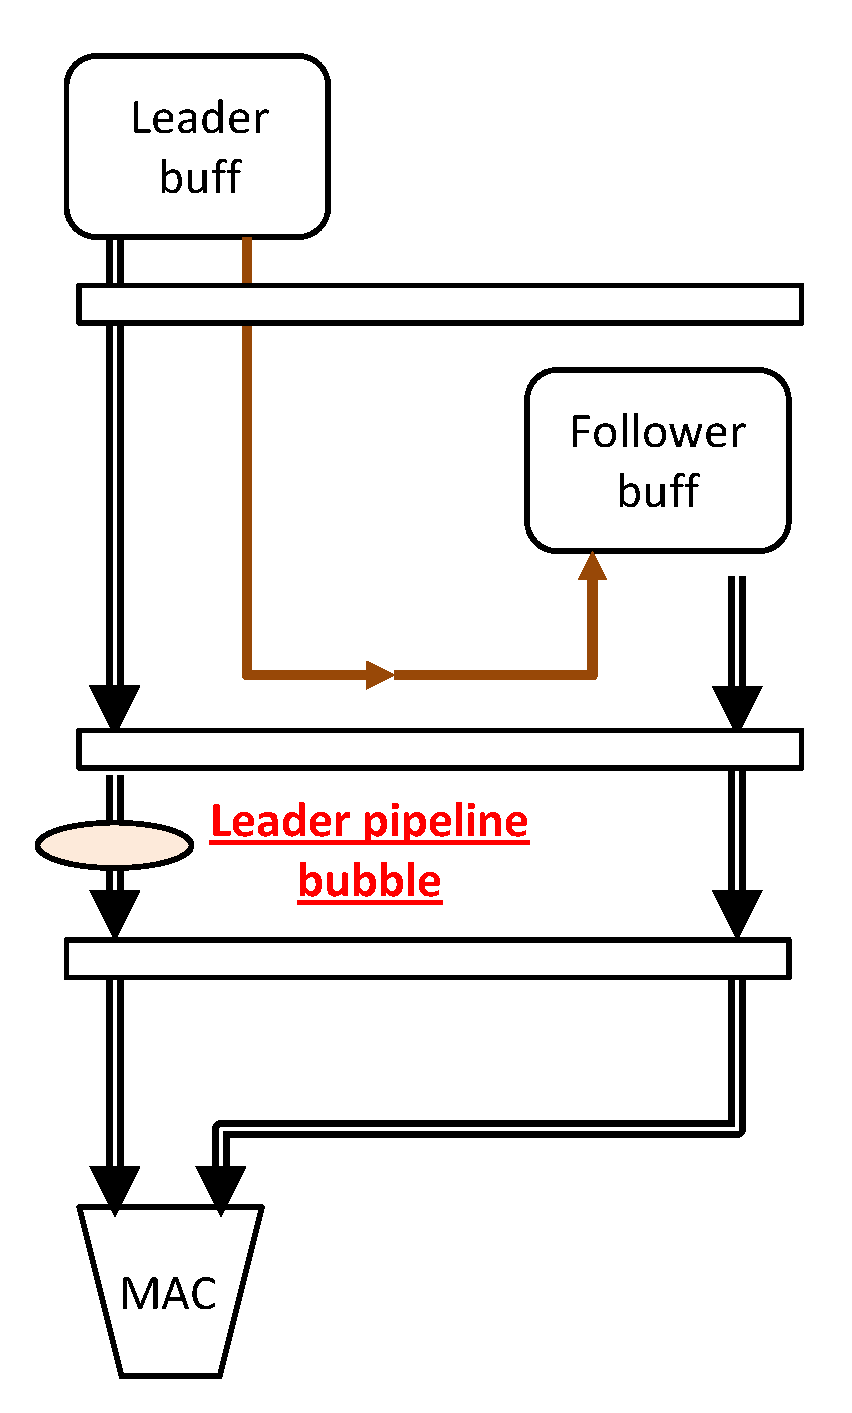
\includegraphics[width=0.6\textwidth]{figures/pipeline_bubble.pdf}
    \caption{Eyeriss v2\cite{eyerissv2}-style pipeline-bubble-based fill optimization.}
    \label{fig:pipeline_bubble}
\end{figure}

\section{Overview of conceptual framework proposed in this work}

\begin{figure}[ht]
    \centering
    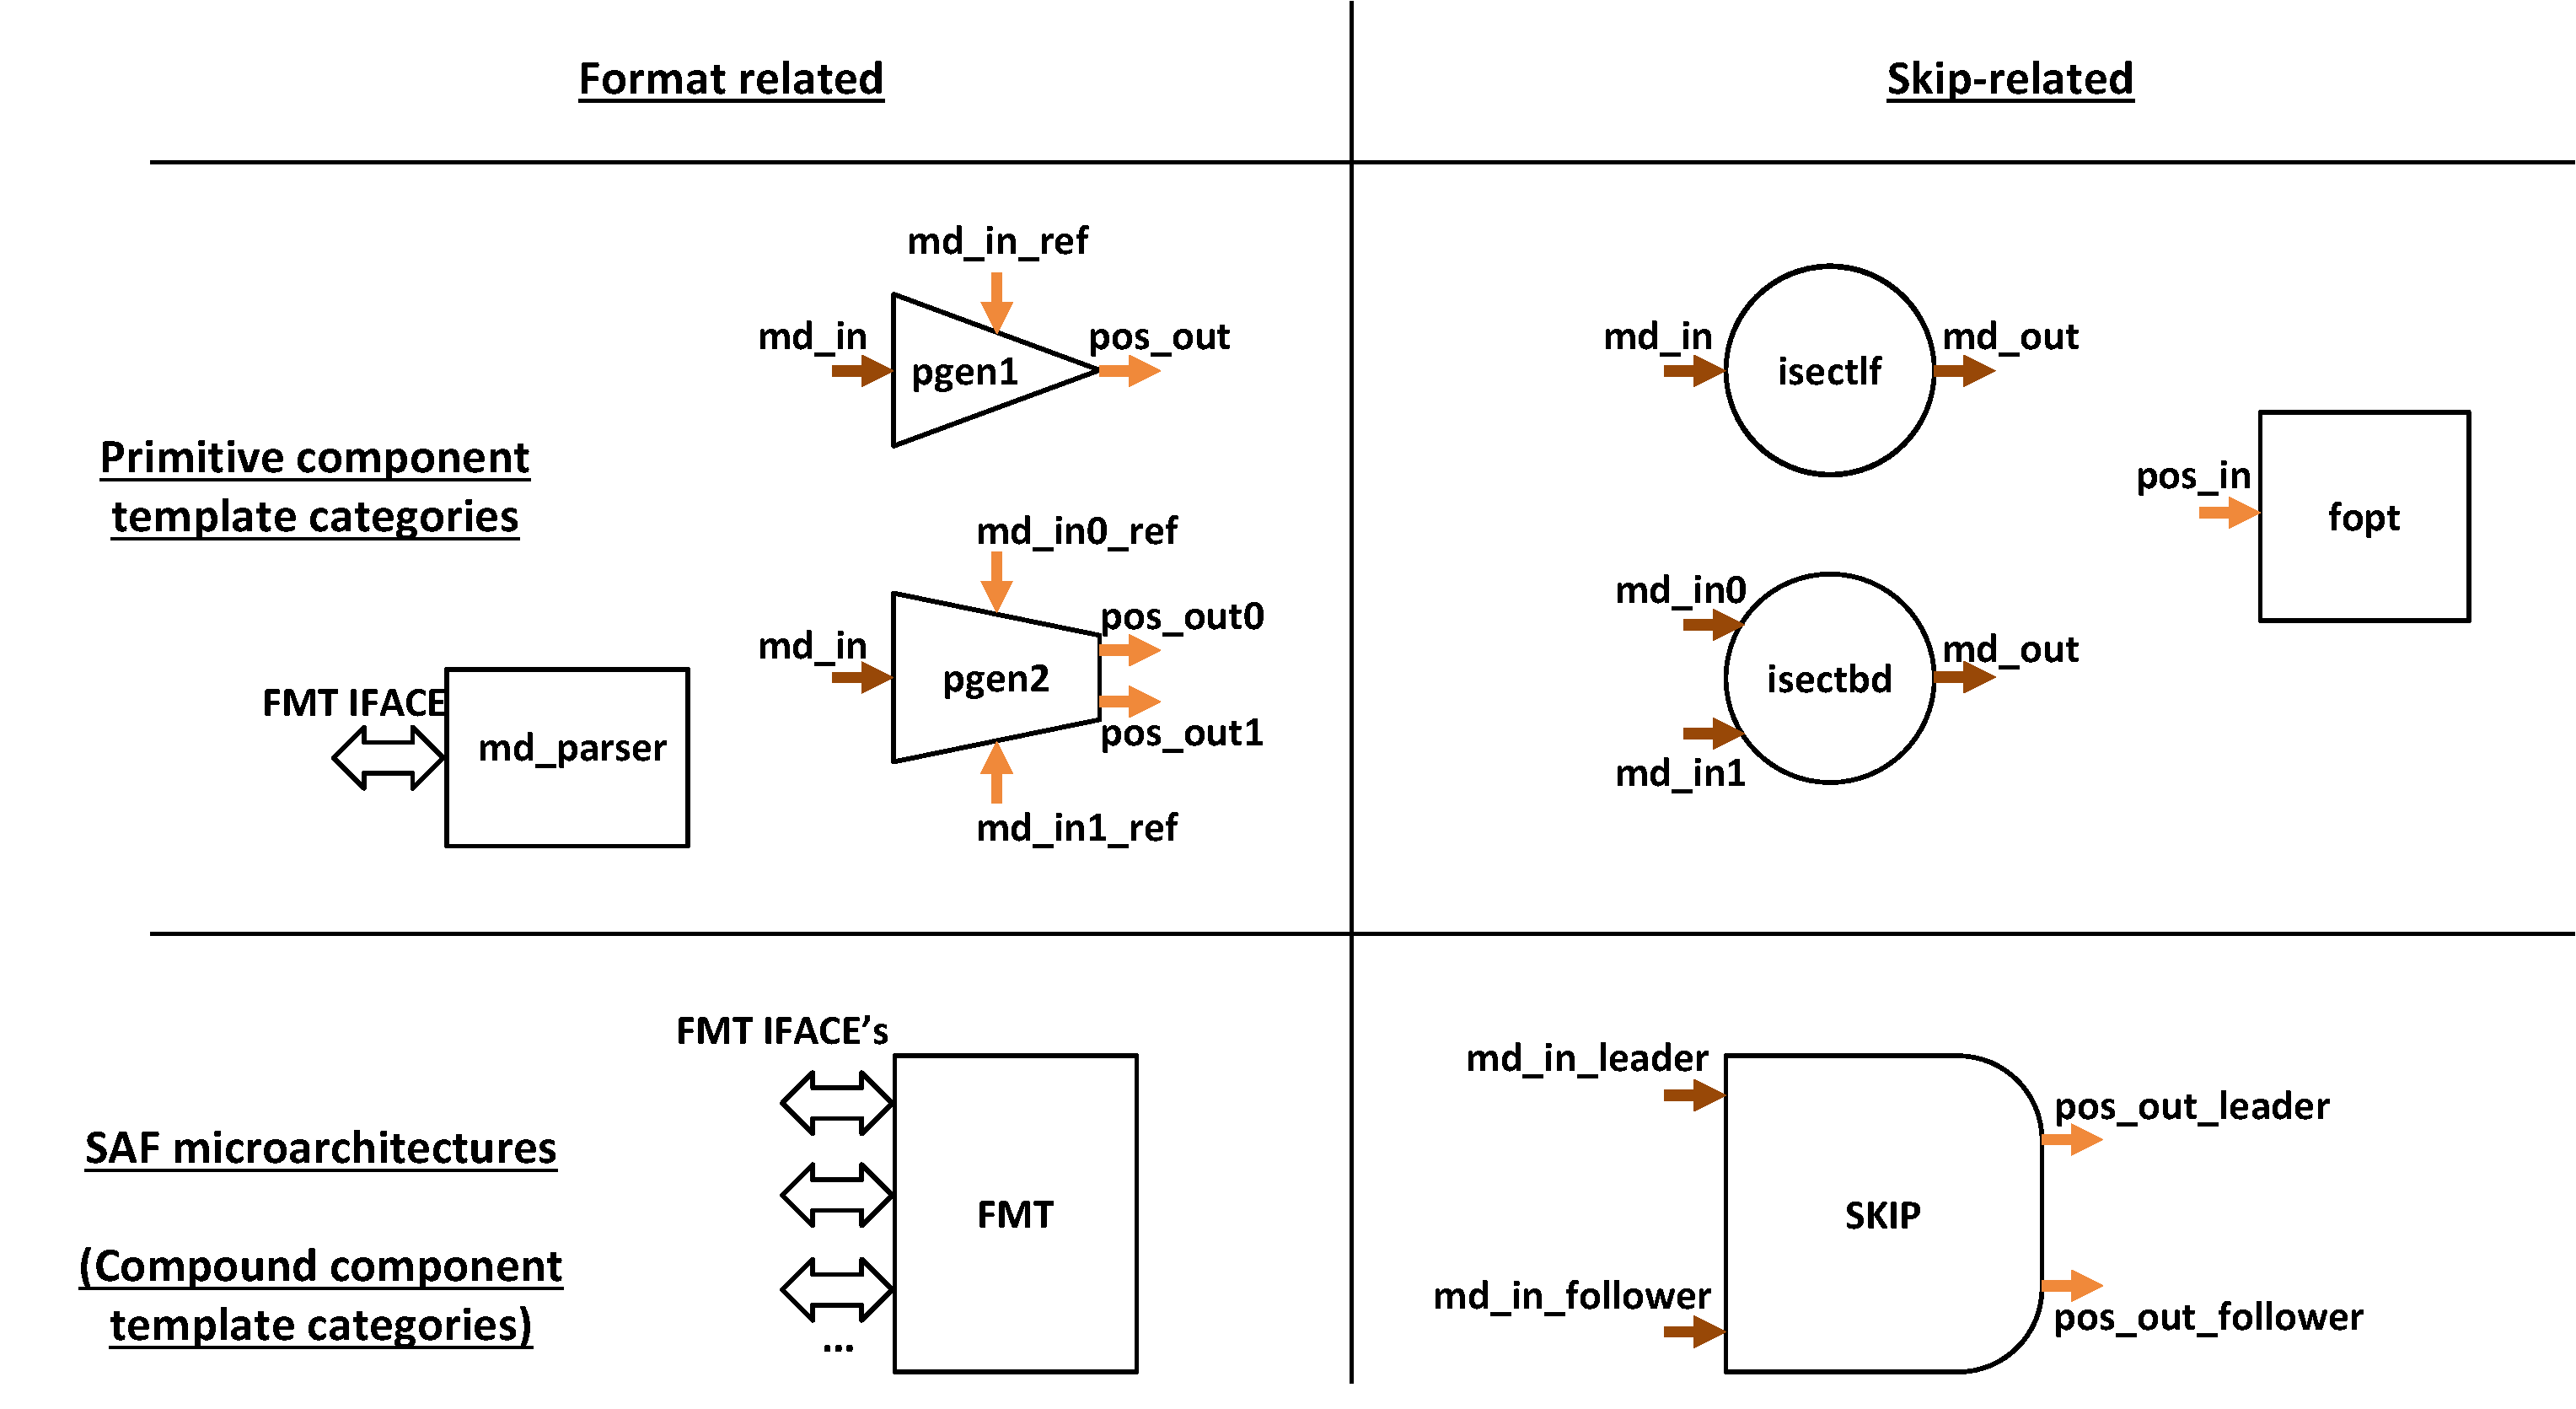
\includegraphics[width=0.95\textwidth]{figures/this_work_taxo.pdf}
    \caption{Overview of the SAF microarchitecture taxonomy developed in this work.}
    \label{fig:this_work_taxo}
\end{figure}

